\documentclass[extra,mreferee]{gji}
\usepackage{timet,amsmath,listings,multirow,graphicx,subfigure,subfig,amsfonts,ulem,xcolor,tikz}
%ulem,amsmath,listings,multirow,array,tikz,amsfonts
\pdfminorversion 4
\newcommand{\btx}{\textsc{BibTeX}}
\renewcommand{\thefootnote}{\fnsymbol{footnote}}
\newcommand{\rs}[1]{\mathstrut\mbox{\scriptsize\rm #1}}
\newcommand{\rr}[1]{\mbox{\rm #1}}
\newcommand{\old}[1]{{\color{red}{\sout{#1}}}{}}
\newcommand{\new}[1]{{\color{blue}{#1}}{}}
\newcommand{\rome}[1]{\romannumeral #1}
\newcommand{\Rome}[1]{{\bf\uppercase\expandafter{\romannumeral #1\relax}}}
\newcommand{\bsy}[1]{\boldsymbol{{}#1}}
\begin{document}
\title[Elastic reflection kernel analysis and traveltime inversion]{Elastic wave-equation-based reflection kernel analysis and traveltime inversion using wave mode decomposition}
\author[Wang et al.]{
	T.F. Wang$^1$, J.B Cheng$^{1,2,*}$, Q. Guo$^3$ and C.L. Wang$^1$\\
    $^1$ School of Ocean and Earth Science, Tongji University, Shanghai,
    China. E-mail: 1110701@tongji.edu.cn\\
    $^2$ State Key Laboratory of Marine Geology, Tongji University,
    Shanghai, China. E-mail: cjb1206@tongji.edu.cn\\
    $^3$ 
	Department of Physical Science and Engineering, King Abdullah University of
	Science and Technology, \\Thuwal 23955-6900, Saudi Arabia\\
    $^*$ Corresponding author: Jiubing Cheng, Shanghai, China. E-mail: cjb1206@tongji.edu.cn\\
}
\date{in original from 2017 August 7}
\maketitle

\begin{summary}
Elastic reflection waveform inversion (ERWI) utilizes the reflections to update the low and
intermediate wavenumber in the deeper part of elastic model, which can provide good initial models
for elastic full waveform inversion (EFWI). Though ERWI can mitigate the nonlinearity to some
extent, it is still stuck with the cycle-skipping problem due to the objective function of waveform fitting. 
Building initial P and S wave velocity models for EFWI through elastic wave-equation
reflections traveltime inversion (ERTI) would be effective and robust
since traveltime information relates to the background model more linearly. 
The wave mode decomposition, both on the recording surface and in the underground space, are important for ERTI.
On the one hand,
P/S separation of multicomponent seismograms on the surface provides 
individual P or S wave data residuals.
Thus, we implement the ERTI using the $L_2$ norm of the isolated P or S wave traveltime
residuals extracted by the dynamic image warping (DIW) as objective function.
On the other hand, the underground spatial wave mode decomposition provides separated wavefields to precondition
the kernels or gradients.
However, the reflection kernels in elastic media are complicated and difficult to use, especially when
calculating the gradient of S-wave
velocity. The investigation of reflection kernels show that mode decomposition can suppress the artifacts in
gradient calculation.
Accordingly, a two-step inversion strategy is adopted to effectively reduce the nonlinearity of inversion, in which PP reflections are first used to invert $V_p$,
followed by $V_s$ inversion with PS reflections based on the well recovered $V_p$.
Numerical example of Sigsbee2A model validates the effectiveness of the
algorithms and strategies for ERTI.
\end{summary}

\begin{keywords}
Inverse theory, Waveform inversion, Elasticity, Seismic tomography
\end{keywords}
\section{Introduction}
With the emergence of long-offset wide-azimuth acquisitions and broad-band sources,
full waveform inversion (FWI) has been recognized as an
efficient tool for constructing velocity models and quantitative seismic imaging, see
\cite{virieux2009overview} for a review.
Though the acoustic FWI, primarily focusing on P-wave velocity inversion, has been
widely studied in the past decades
\cite[]{tarantola1984,pratt1998gauss,shipp:2002}, people are paying more attention
to the waveform inversion under the elastic assumption, referred to as elastic full waveform inversion
(EFWI) \cite[]{tarantola1986}.
Waveform inversion provides high-resolution model estimation of the elastic
properties, but it
suffers from the cycle-skipping easily because of its insensitivity to the low and intermediate wavenumber components of the model
when the acquisition illumination is poor and/or good initial models are unavailable during the inversion\cite[]{sears2008,brossier2009}.
Besides, multi-parameter trade-off effects and more complicated elastic wave phenomena
will further increase the difficulties for EFWI.
To deal with the nonlinearities and parameter trade-offs, more
preconditioning, hierarchical strategies and parameterization investigation should be
considered during EFWI
\cite[]{sears2008,prieux:2013b,operto2013guided,wang:2015,Oh2016}.

%In the surface observation geometry, full waveform inversion (FWI) often suffers from the
%local minimal due to the absence of low frequencies in the data when the low-wavenumber
%component is missing in the initial model.
For the classical FWI, the long-offset data
corresponding to diving waves are very important to build the long-to-intermediate
wavelengths of the model. However, the penetration depths of
diving waves are always far from sufficient to reach the target in the deeper part
%with the limited surface offset,
even using the wide-aperture surveys.
In addition, the low signal-to-noise ratio at the far
offset is also a limit for the classical FWI relying on the diving waves.
Therefore, people tried to utilize the reflections
to help build the macro-model containing low-to-intermediate wavenumber
in the deep part\cite[]{Stork1992,ChaventEtAl1994,clement:2001,Symes2008a,xu:2012}.
This process can be implemented in the image domain or the data domain.
Actually, the image-domain ray-based tomography
\cite[]{Stork1992,Woodward1992,Woodward2008,Jones2010} has already been a standard workflow to obtain the background velocity by flatting the common
image gathers. But when the lateral velocity variation is strong, the ray-based method would fail to
present the wave propagation underground.
%, which will probably lead to the failure of tomography. 
To overcome the limit of ray theory,
people have made great efforts to develop the approaches of reflection inversion that employ
waveform or traveltime information based on wave-equation
\cite[]{xu:2012,Ma2013,Wu2015b,Zhou2015,Wang2015,Chi2015}.

The misfit function of reflection inversion can be built in image domain in the manner of wave equation migration
velocity analysis (WEMVA), which tries to maximize the
energy at zero-offset location in the extended subsurface image gathers
\cite[]{Symes2008,Almomin2012,SunEtAl2012,biondi2013}.
%Alternatively, the image domain strategy also can be fulfilled by the wave equation
%migration velocity analysis (WEMVA), in which velocity is updated
%through minimizing the energy of non-zero offset on the extended-domain gathers \cite[]{Symes, 2008; Fleury
%and Perrone, 2012; Biondi and Almomin, 2013}.
\cite{RaknesEtAl2016}
developed an image-domain method to invert P-wave velocity ($V_p$) in the 3D elastic media.
\cite{Wang2017WEMVA} proposed to employ the extended PS image in WEMVA to update the
S-wave velocity ($V_s$) with the help of elastic wave mode decomposition.
%But it is a big issue that the extended domain approach requires huge computational cost,
%especially in 3D case.
However, the extended-domain methods are limited due to its prohibitively computational cost,
especially in 3D case.
While in the data domain,
\cite{xu:2012} suggested using a reflection waveform inversion (RWI) method to suppress the
nonlinearity in FWI,
which aim to invert the long-wavelength components of the model by using the reflections
predicted by migration/demigration process.
Recently, \cite{Zhou2015} proposed a joint FWI method that combines the diving and reflected waves to
utilize both RWI and the conventional FWI.
\cite{Wu2015b} developed an RWI scheme to simultaneously invert the background velocity and the
perturbation in acoustic media,  and recently extended to elastic case by
\cite{Guo2016}.
RWI highly relies on the accurate reflectivity to generate the reflections that can match the
observed data. However, it is very challenging and also expensive to obtain a good reflectivity model through
least-square migration when initial model is far away from the true one.

%In addition, \cite{Wang:2015} found that wave mode decomposition may be beneficial to deal with the
%elastic parameter trade-offs.
Compared with the waveform information,
%traveltime is more sensitive and linearly related to
%low-wavenumber model perturbation. Using traveltime inversion will be more robust and helpful to
%build appropriate initial models containing long-wavelength components for
%conventional FWI \cite[]{Ma2013, Wang2015,Chi2015, Luo2016}.
traveltime is more sensitive and linearly related to
the low-wavenumber components of the model. Therefore, traveltime inversion will be more robust and helpful to
build good initial models for conventional FWI
\cite[]{WangEtAl2014}.
\cite{Ma2013} introduced a wave equation reflected traveltime inversion method
based on dynamic image warping (DIW) to build the low wavenumber of the model.
\cite{Chi2015} and \cite{Wang2015} employed correlation-based method to extract the
temporal or spatial lag to implement the reflection inversion.
Elastic reflections carry the background information of the P and S wave velocities,
which can help to rebuild the good initial velocity models for EFWI.
Unfortunately, in elastic case, traveltime shifts of a particular wave mode are difficult
to extract due to the complicated wave phenomenons, such as mode-conversions.
%It is common to observe that different mode-conversions, mainly P-P
%and P-S events, overlap and intersect with each other. The cross points between events
%would be singularities for traveltime difference estimation even using the local shift estimation 
%method like DIW.
Therefore, the estimated time shifts would be inaccurate if using the
original multicomponent seismograms directly.
%, which makes the elastic wave-equation reflection
%traveltime inversion (ERTI) difficult to implement.
In addition, since the multi-parameter trade-offs will increase the
nonlinearity of inversion, more hierarchical strategies should be considered to deal
with this problem.
\cite{WangEtAl2017}
preconditioned the gradients of EFWI through wave mode decomposition to mitigate
parameter trade-offs and explained that this precondition employs the off-diagonal Hessian blocks
when inverting $V_s$.
As a natural tool to obtain the separated data subsets, the wave mode decomposition similarly
has the potential to precondition the elastic wave-equation reflection traveltime
inversion (ERTI) with more flexible hierarchical strategies.

%In this paper,
%we aim to tackle the traveltime misfits of P-P and P-S reflections with the help
%of wave mode decomposition and dynamic image warping (DIW) \cite[]{Hale2013}.
%Then, we use the traveltime of P-P and P-S reflections to implement the 
%WERTI method \cite[]{Ma2013} with a two-stage workflow.
%Finally, the numerical example of Sigsee2A model proves the robustness and validity of our
%elastic WERTI method.


%The key point of RWI is to project the data-domain residuals back to the reflection wavepath to 
%is to project the data-domain residuals back to the reflection wavepath to 

%for both the imaging condition and the forward modelling in each iteration.

%\cite{Zhou2015} proposed a joint FWI method to combine the diving and reflected waves to
%utilize both the conventional FWI and RWI.
%In addition, \cite{Wang:2015} found that wave mode decomposition may be beneficial to deal with the
%elastic parameter trade-offs.
%build appropriate initial models containing long-wavelength components for
%Unfortunately, in elastic case, traveltimes of a particular wave mode are difficult
%to extract due to the complicated mode-conversions. 

In this paper,
we will exploit the traveltime misfits of PP and PS reflections to implement the ERTI
approach with the aid
of wave mode decomposition and DIW \cite[]{Hale2013}.
%In this abstract, we separate the PP and PS reflections in the observed and predicted multicomponent data to
%extract the individual traveltime residuals through DIW \cite[]{Hale2013}.
%using surface P/S wave
%separation. Dynamic image warping \cite[]{Hale2013} helps to extract the local traveltime residual
%between the observed and the predicted data.
First,
the elastic reflection kernel and its components of different wave modes are
calculated and the implications to suppress the artifacts in the gradient calculation
are investigated.
%to investigate  the effectiveness of mode decomposition on suppressing the artifacts in the gradient calculation.
Then, P/S separation of multicomponent seismograms is applied to the observed and predicted reflection data
to extract the individual traveltime residuals of PP and PS reflections through DIW.
Based on the analysis of elastic reflection kernels and the separated traveltime residuals,
we design a two-stage workflow to implement
the ERTI method,
in which the traveltime of PP reflections are firstly used to recover the background
$V_p$ model and then the traveltime of PS reflections are used to recover the background $V_s$ model
.
According to our investigation, it is not suitable to estimate the time shifts of PS
reflections at near offset if we
use the PS image to predict the corresponding reflection during demigration.
Instead, we recommend to use PP image to do that.
%During the $V_s$ inversion, the PS reflections are predicted by the PP image to avoid
%the wrongly estimated time shifts when using PS image.
Moreover, we precondition the $V_s$ gradient through the spatial wave mode
decomposition.
Finally, the numerical example of Sigsee2A model proves the robustness and validity of our
ERTI method.

\section{Theory of ERTI}
Assume that there is a perturbation $c^{1}_{ijkl}$ in the background elastic media
$c^0_{ijkl}$, using the Born approximation, the background wavefields $u_i$ and perturbed wavefields
$\hat{u}_i$ satisfy:
\begin{equation}
    \rho \frac{\partial u^2_i}{\partial t^2}  -
    \frac{\partial}{\partial x_j}\left[ 
        c^0_{ijkl}\frac{\partial u_{k}}{\partial
        x_l}\right]=f_i,
    \label{eq:WE} 
\end{equation}
and
\begin{equation}
	\rho \frac{\partial \hat{u}^2_i}{\partial t^2}  -
    \frac{\partial}{\partial x_j}\left[ 
	c^0_{ijkl}\frac{\partial \hat{u}_{k}}{\partial
        x_l}\right]=\frac{\partial}{\partial x_j}\left[c^1_{ijkl}\frac{\partial u_{k}}{\partial x_l}\right],
    \label{eq:DeltaWE} 
\end{equation}
in the sense of first-order elastic scattering, where $\hat{u}_i$ can be taken as the demigrated reflection data using the image
perturbation $c^1_{ijkl}$ obtained from reverse time migration (RTM) or other imaging method. In ERTI, we
aim to minimize the traveltime differences (or time shifts) between the observed data
$\mathbf{d}^{o}$ and
the calculated data $\mathbf{d}^{c}$, using the following  
objective function: 
%\begin{equation}
%	E=\frac{1}{2}\int\tau^2(\mathbf{x_r},t;\mathbf{x_s})dtd\mathbf{x_r}d\mathbf{x_s},
%    \label{eq:Objectivefunction} 
%\end{equation}
\begin{equation}
	\left\{
		\begin{aligned}
			&\tau(\mathbf{x_r},t)=\mathop{\arg\min}_{\tau}
			\int^T_0\sum_r\parallel\mathbf{d}^{c}(\mathbf{x}_r,t)-\mathbf{d}^{o}(\mathbf{x}_r,t+\tau)\parallel^2\\
    &E=\frac{1}{2}\int^T_0\sum_r\tau^2(\mathbf{x_r},t)dt,
		\end{aligned}
	\right.
    \label{eq:Objectivefunction} 
\end{equation}
where the time differences $\tau(\mathbf{x_r},t)$ can be extracted
through DIW (The readers can refer to \cite{Hale2013} for detail).

After the derivation in Appendix A using the adjoint state method, the gradients of equation \eqref{eq:Objectivefunction} can be expressed as:
\begin{equation}
	\frac{\partial E}{\partial c^0_{ijkl}}=-\int (\frac{\partial u_{i}}{\partial
	x_j}\frac{\partial \hat{\psi}_{k}}{\partial x_l}+\frac{\partial \hat{u}_{i}}{\partial
	x_j}\frac{\partial \psi_{k}}{\partial x_l}),
    \label{eq:GradientCijkl}
\end{equation}
where $u_i$ and $\hat{u}_i$ are the state variables, representing the forward
background wavefields and the perturbed wavefields, respectively. While $\psi_i$ and $\hat{
\psi}_i$ are the adjoint state variables, representing the back-propagated background
wavefields and the perturbed wavefields, satisfying:
\begin{equation}
    \rho \frac{\partial \psi^2_i}{\partial t^2}  -
    \frac{\partial}{\partial x_j}\left[ 
        c_{ijkl}\frac{\partial \psi_{k}}{\partial
		x_l}\right]=\tau(\mathbf{x_r},t)\frac{\dot{d}^o_i(\mathbf{x_r},t+\tau)}{h_i(\mathbf{x_r},t)},
    \label{eq:AdjointWE} 
\end{equation}
and
\begin{equation}
    \rho \frac{\partial \hat \psi^2_i}{\partial t^2}  -
    \frac{\partial}{\partial x_j}\left[ 
        c_{ijkl}\frac{\partial \hat\psi_{k}}{\partial
        x_l}\right]=\frac{\partial}{\partial x_j}\left[\delta c_{ijkl}\frac{\partial
		\psi_{k}}{\partial x_l}\right],
    \label{eq:AdjointDeltaWE} 
\end{equation}
with
$h_i(\mathbf{x_r},t)=\dot{d}^o_i(\mathbf{x_r},t+\tau)^2-\ddot{d}^o_i(\mathbf{x_r},t+\tau)(d^c_i(\mathbf{x_r},t)-d^o_i(\mathbf{x_r},t+\tau)$.
The hat dot denotes the time derivative. On the right hand side of equation
\eqref{eq:GradientCijkl}, the two terms indicate two cross-correlations that represent the source and receiver
parts of the reflection wavepath, respectively. For simplicity, we derive the
gradients of stiffness
coefficients for inversion. But the velocity parameterization will be more reasonable
to implement the traveltime inversion.
Thus, we get the gradients in terms of P- and S- wave velocities through the chain rule, namely:
\begin{equation}
	\begin{split}
	&\frac{\partial E}{\partial V_p}=2\rho V_p\frac{\partial E}{\partial
		c^0_{ijkl}}\delta_{ij}\delta_{kl}, \\
	&\frac{\partial E}{\partial V_s}=2\rho V_s\frac{\partial
	E}{\partial c^0_{ijkl}}(-2\delta_{ij}\delta_{kl}+\delta_{ik}\delta_{jl}+
	\delta_{il}\delta_{jk}).
	\end{split}
    \label{eq:GradientVel}
\end{equation}

\section{Elastic Born reflection kernels}
Reflection traveltime and waveform inversions utilize different objective functions
but share the same reflection wavepath information (reflection kernels). 
%From the perspective of gradient calculation, different objective functions only induce different types of adjoint
%sources. 
Therefore, the key point of reflection inversion is how to calculate and utilize the reflection kernel. 
%Different types of objective funtion only induce different types of adjoint sources.
For simplicity, we rewrite \eqref{eq:GradientCijkl} as follow:
\begin{equation}
    \nabla E(
    \mathbf{m}_0)=-\int(
    \mathbf{u}\otimes\bsy{\hat\psi}
    +
	\mathbf{\hat{u}}\otimes{\bsy{\psi}})
    \label{eq:kernelgradient} 
\end{equation} 
with $\mathbf{m}_0$ is the background model, $\mathbf{u}$ and $\mathbf{\hat{u}}$ are the incident
and perturbed forward wavefields,
 while $\bsy{\psi}$ and $\bsy{\hat\psi}$ are the incident and perturbed adjoint wavefields,
 respectively.
The operator $\otimes$ denotes the cross correlation between two wavefields. 
Note that, equation \eqref{eq:kernelgradient} just schematically shows the manner of cross correlation. 
The detailed formulas should be derived according to the parameterization through
chain rule as in equation \eqref{eq:GradientVel}.

In elastic case, due to the complex wave phenomena, the four wavefields in eq.
\eqref{eq:kernelgradient} contain both P and S waves, then the cross-correlations between
different wave mode conversions will generates cross-talks in the kernel \cite[]{Wang2017ERTI}. Therefore, the wavepath of elastic reflections will 
be far more complicated than that in acoustic case.
%Since in the elastic case, the four wavefields in eq. \eqref{eq:kernelgradient} contain both P and S
%waves, the cross-correlation between different wave modes may cause interference to
%gradients \cite[]{Wang2017ERTI}.
To analyze the elastic reflection kernels, 
we decompose the original kernel into four components which 
correspond to the cross-correlation of different wave modes, respectively, as follows:
%Tthe above formula can be decomposed into four types with:
\begin{equation}
    K_{m_0}^{MN}     
    =-\int(\mathbf{u}^M\otimes\bsy{\hat\psi}^N
	+\mathbf{\hat{u}}^M\otimes\bsy{\psi}^N),\\
    \label{eq:decompkernel} 
\end{equation}
where $M,N\in\{P,S\}$.
$K_{m_0}^{MN}$ represents the cross correlation between the $M$ mode forward wavefields and the 
$N$ mode adjoint wavefields. 
For example, $K^{PS}$ is the
cross-correlation of P-mode forward wavefield and S-mode adjoint wavefields. So the $M$ or $N$ is
the mode type of the wavefields involved in cross-correlation but not 
the mode type of shot data.
As illustrated in Fig. \ref{fig:kernel_mirror_src}, this
kernel can be considered as the cross-correlation between the forward wavefields
emitted from a virtual source at a mirror location and the adjoint wavefields
back-propagated from the receiver. If the traveltime of the adjoint wavefields (injected at
receiver) is consistent with the forward wavefields, the cross-correlation will
produce the low-wavenumber wavepath. Otherwise, the cross-correlation
should be a high-wavenumber migration impulse. 
%Note, it does not denote the kernel of $MN$ mode data. For example, the reflection 
%kernel of PS data should be $(\mathbf{u}^P\cdot\delta \bsy{\psi}^P +\delta
%\mathbf{u}^S\cdot\bsy{\psi}^S)$ but not $K^{PS}$.

For instance, we calculate the kernels with the single-source-receiver data
which are synthesized for a single reflector with a pure P-wave source.
%Here we use a waveform data residual as the adjoint source for back-propagation.
Since different objective functions only induce different types of adjoint
sources from the perspective of gradient calculation, we can investigate the reflection kernel 
using the waveform data residual as the adjoint source for back-propagation.
%We use the $V_p$ - $V_s$ parameterization as in equation \eqref{eq:GradientVel}.
In the first test, we place a single $V_p$ reflector in the homogeneous background
(Figs \ref{fig:kernel1_vp}a and b). 
%We use the single source-receiver reflection data to calculate the kernel.
Since there is no perturbation of $V_s$, only PP reflection exist in the data (almost
the same as in acoustic media), which means mode decomposition is unnecessary in this
case.
As shown in Figs \ref{fig:kernel1_vp}c and d, the reflection
kernel consists of two ``rabbit-ears'', the
source and receiver parts. $K_{V_p}$ produces the low-wavenumber PP reflection
wavepath as expected.
While in $K_{V_s}$, the energy focus on the edge of the wavepath rather than the first Fresnel-Zone as in the $V_p$ kernel.
One plausible reason is that the $V_s$ kernel is relatively insensitive to the PP data generated by $V_p$ reflector.
Besides, we can see the migration impulse below the reflector due to the down-going perturbed wavefields.


In the second test, we use the $V_s$ reflector (Figs \ref{fig:kernel2}a and
b) to generate both PP
and PS reflections.
%The $V_s$ reflector produces both PP and PS data. 
The $V_p$ kernel excludes S-wavefield automatically because of the divergence operator 
implied in the term $\delta_{ij}\delta_{kl}$, see eq. \eqref{eq:GradientVel}. 
However, $\bsy{\hat\psi}$ contains the converted SP wavefields 
induced by the back-propagated  $\bsy{\psi}^S$ at the location of reflector.
These non-physical wavefields make the $V_p$ kernel slightly different from that in
Fig. \ref{fig:kernel1_vp}c.
To remove these non-physical artifacts in $K_{V_p}$, we should only inject the PP data during the
back-propagation. 
%If we only back-propagate the PP data, $V_p$ kernel will be the same as Figure \ref{fig:kernel1_vp}c.

For the $V_s$ kernel (Fig. \ref{fig:kernel2}d), due to mode conversions, multi-wavepaths overlapping with each other 
make it much more difficult to calculate and exploit the correct reflection kernel. 
The straightforward utilization of this kernel in gradient calculation will very likely cause 
cross-talk during reflection inversion.
According to equation
\eqref{eq:decompkernel}, we calculate the components of $K_{V_s}$, as shown in Fig.
\ref{fig:kernel2_vs_decomp}. We observe that the $K^{PP}_{V_s}$ is similar to $K^{PP}_{V_p}$ but with an opposite
sign. This is because the term $\delta_{ij}\delta_{kl}$ implied divergence operator has
a negative sign in the $V_s$ gradient (eq. \eqref{eq:GradientVel}).
$K^{PS}_{V_s}$ and $K^{SP}_{V_s}$ mainly consist of high-wavenumber energy
corresponding to the migration impulse of cross-mode wavefields. 
Fig. \ref{fig:kernel2_vs_decomp}d shows that the
separated S-wavepath of PS reflection is little affected by the P-wavefields. 
%S-wave part of the PS reflection wavepath. 

To further investigate the implication of the reflection kernel, we will
analyze the generation of every parts by not only decomposing the spatial wavefields
but also isolating the injection of PP or PS data.
Taking the second test as example, we further decompose the kernels into 
several parts by using the manner shown in the schematic illustrations, respectively. 
The decomposition of $K_{V_p}$ is easy to understand 
(Fig. \ref{fig:kernel_vp_decomp}) 
because only $K^{PP}$ is involved. In Fig
\ref{fig:kernel_vp_decomp}e, only the PP data are injected as adjoint source, then the
cross-correlation between
perturbed wavefields $\bsy{\hat\psi}^{PP}$ and the background
$\mathbf{u}^P$ produces a clean PP wavepath at the source side. The	schematic
illustration with raypaths denotes the wave mode of
the modelled and adjoint wavefields involved in the calculation. Note that,
when PS data are back-propogated, an SP conversion will
occur at the interface, which will produce a migration impulse, as shown in
Fig. \ref{fig:kernel_vp_decomp}f. Moreover, in
Fig. \ref{fig:kernel_vp_decomp}h, 
since a non-physical P wavefield is generated in $\bsy{\psi}$ due to the PS data injection
\cite[]{Ravasi2013}, 
another migration impulse can be seen at the receiver side. 
Accordingly, the non-physical conversions related to the PS data injection will
cause artifacts in the $K_{V_p}$ calculation. 

Since $K_{V_s}$ is more complicated, we first decompose it into  source and receiver
parts as shown in Figs \ref{fig:kernel_vs_decomp}c and d. Then, the isolation of PP
and PS data injection provides four different components, respectively
(Figs \ref{fig:kernel_vs_decomp}e to h).
Figs \ref{fig:kernel_vs_decomp}e and f show the decomposition of
the kernel in Fig. \ref{fig:kernel_vs_decomp}c
while Figs \ref{fig:kernel_vs_decomp}g and h corresponds to the decomposition of the kernel in Fig.
\ref{fig:kernel_vs_decomp}d.
These four components can be further decomposed with the help of mode decomposition. 
For simplicity, we will only analyze the decomposition of  Fig. \ref{fig:kernel_vs_decomp}h,
while the analyses of the rest three parts will be placed in Appendix B.
In Fig. \ref{fig:kernel_vs_recPS}, 
P and S wavefields are
generated simultaneously in $\bsy{\psi}$ when PS data is injected. 
Although \ref{fig:kernel_vs_recPS}c denotes a same-mode correlation, 
it generates a migration impulse 
due to the  inconsistent traveltime of modelled $\mathbf{\hat{u}}^{PP}$ and non-physical
converted $\bsy{\psi}^{P}$, as if a PP event is injected at the location of PS event.
The cross-mode correlations in 
Figs \ref{fig:kernel_vs_recPS}d and e
also produce migration impulses. 
Luckily, the cross-correlation between $\bsy{\psi}^{S}$ and $\mathbf{\hat{u}}^{PS}$ provides the
low-wavenumber S-wavepath of the PS reflection.

According to the above investigation, we know that the cross-correlation between
different wave modes cause cross-talks in gradient calculation. The injection of separated PP
reflection data helps to reduce the artifacts in $V_p$
gradients, so does the injection of separated PS reflection data for $V_s$ gradient calculation.
Most importantly, we expect to update the $V_s$ model through the S-wavepath in PS reflection, which is
exactly the component $K^{SS}_{V_s}$.  
Therefore, we recommend using $K^{SS}_{V_s}$ to mitigate the cross-talks in $V_s$ gradient calculation.

\section{Workflow of elastic WERTI}
In elastic case, it is common to observe that different mode-conversions, e.g. PP
and PS events, overlap and intersect with each other in the original multi-component
seismograms . The cross points between events
would be singularities for traveltime difference estimation through DIW.
%DIW extracts the reflection traveltime differences in data domain. In elastic case, %PP and PS reflections 
%the cross points between different mode-conversions would be singularities for DIW.
Therefore, the estimated $\bsy{\tau}(\mathbf{x_r},t)$ would be inaccurate due
to these singularities.
%if using the original multicomponent seismic data, which makes equation \eqref{eq:GradientVel} difficult to implement.
Moreover, according to the reflection kernel analysis, individually injecting separated
PP or PS seismograms
can mitigate the cross-talk in gradient calculation. 
Thus, we decompose the observed and synthesized data into P- and S-wave
parts through P/S separation of multi-component seismograms \cite[]{Li2016a}.
In this way, 
it is relatively easier to estimate the time shifts through DIW for PP and PS reflection,
respectively.
%the traveltime differences can be decoupled into PP and
%PS parts by DIW. 
Accordingly, we implement the ERTI through a two-stage
workflow, i.e. estimating $V_p$ using PP reflections followed by estimating $V_s$ 
using PS reflections.

\subsection{Stage \Rome{1}: ERTI of PP reflection}
In this stage, we use traveltimes of PP reflection to recover the low-to-intermediate wavenumbers of
the $V_p$ model. 
The perturbation of $V_p$ ($\delta V_p$) is obtained through elastic reverse time migration (ERTM). 
When the migration velocity model is inaccurate, 
%the migration/demigration of large-offset data would produce deviated
%zero-offset two-way travletime, which will increase the nonlinearity of inversion.
%Therefore, 
people always take
the two-way travletime of zero-offset as an invariants during reflection inversion, such as reflection traveltime tomography or RWI,
and thus use the zero or small offset data to generate the velocity perturbation \cite[]{Zhou2015}. 
Nonetheless, this method still may fail to ensure a correct zero offset traveltime in the
demigration when velocity anomaly is complex. A better method would be the demigration with the extended
image \cite[]{Weibull2014, Hou2015, Qiang2017}, but it is out of the scope of this paper.
Besides, since the traveltime rather than the amplitude is fitted in ERTI, 
ERTM (instead of its least-squares counterpart) is sufficient to obtain the image perturbation for
the demigration.
%but not a least-squares manner (LSRTM) to find the correct reflectivity. 
Thus, the objective function can be written as:
\begin{equation}
	\left\{
		\begin{aligned}
			&\tau_{pp}(\mathbf{x_r},t)=\mathop{\arg\min}_{\tau}
			\parallel\mathbf{d}^{c}_{pp}(\mathbf{x}_r,t)-\mathbf{d}^{o}_{pp}(\mathbf{x}_r,t+\tau)\parallel^2\\
			&E_{pp}=\frac{1}{2}\int\tau^2_{pp}(\mathbf{x_r},t)dtd\mathbf{x_r},
		\end{aligned}
	\right.
    \label{eq:ObjectivefunctionPP} 
\end{equation}
where $\mathbf{d}^{c}_{pp}$ and $\mathbf{d}^{o}_{pp}$ are synthesized and observed PP reflection after the P/S
separation on the recording surface, respectively. According to the previous derivation, we can
obtain the gradient of  $V_p$, i.e. $\frac{\partial E}{\partial
V_p}$.
Note that, 
the divergence operator is implied in $\frac{\partial
E}{\partial V_p}$, which makes the gradient calculation only involve PP reflection.
%is similar to the $V_p$ gradient of EFWI.
Therefore, the PP reflection traveltime inversion for $V_p$ in elastic media is similar to the acoustic case
except that the isolation of PS component is required in the former one. In addition, the separated
P-wave reflections may include some SP conversions due to the source-side effects in the elastic
case. %This may lead to the mismatch of the traveltime inversion.
\subsection{Stage \Rome{2}: ERTI of PS reflection}
In the second stage, we utilize the PS reflections to retrieve the background component of
$V_s$ model. Similarly, the objective function becomes:
\begin{equation}
	\left\{
		\begin{aligned}
			&\tau_{ps}(\mathbf{x_r},t)=\mathop{\arg\min}_{\tau}
			\parallel\mathbf{d}^{c}_{ps}(\mathbf{x}_r,t)-\mathbf{d}^{o}_{ps}(\mathbf{x}_r,t+\tau)\parallel^2\\
			&E_{ps}=\frac{1}{2}\int\tau^2_{ps}(\mathbf{x_r},t)dtd\mathbf{x_r}.
		\end{aligned}
	\right.
    \label{eq:ObjectivefunctionPP} 
\end{equation}
where $\mathbf{d}^{c}_{ps}$ and $\mathbf{d}^{o}_{ps}$ are synthesized and observed PS reflections, respectively.
After the first stage inversion, both the background model and the structural image 
perturbation of $V_p$ have been well recovered. These are the good constrains for the prediction 
of PS reflection. Moreover, in
most geological settings, $V_p$ and $V_s$ share the same structure in the subsurface. 
It means that we can use the well-located $\delta V_p$ instead of $\delta V_s$ to generate the PS reflections. 
Therefore, to fit the traveltimes, there are two ways to predict the PS reflection:

\Rome{1}: Migrate the observed PS data with inverted $V_p$ model and
initial $V_s$ model to get the high wavenumber of $V_s$ ($\delta V_s$), then predict the PS reflection;

\Rome{2}: Start from the inverted $V_p$ model and initial $V_s$
model, use the well-located $\delta V_p$ as the virtual source to generate the PS reflections. 

%However, the implementation is a little different from the previous stage. 

Unfortunately, the predicted PS reflection with method \Rome{1} are
inconsistent with the error of $V_s$ model at near offset. 
In Appendix C, we illustrate this inconsistency for inversion through a single reflector
example with
map migration and demigration under the high-frequency approximation.
Therefore, we recommend to use method \Rome{2}.
%which will make the inversion more nonlinear.
%The difference between method {\bf\uppercase\expandafter{\romannumeral1}} and {\bf\uppercase\expandafter{\romannumeral1}} is that 
Nonetheless, the amplitude of the predicted PS will be inaccurate when using 
method \Rome{2}, even if $\delta V_p$ is obtained by the
least-squares ERTM. 
Fortunately, the inaccurate amplitude of PS prediction has little effect on ERTI because ERTI only
cares the kinematic information.
Note that 
the traveltime residuals of the PS reflection may be 
large in the deeper part (Fig. \ref{fig:Sens_vp}). DIW may suffer from the cycle-skipping problem in this
situation. We can utilize the ``layer-stripping'' strategy to tackle this, during which the shallow part is
inverted using the early arrived reflection while the deep part is inverted using the late
arrived reflections gradually. In this way, the incorrect traveltime residuals of the deeper part will not
mislead the inversion of shallow part. Vice versa, the reliable inversion of the shallow part
guarantee
the correctness of traveltime residual for the deeper part.

In order to make sure that reflected S-wavepath is used to update $V_s$, the wave mode decomposition 
is applied to calculate $K^{SS}_{V_s}$, namely:
%we drop the first term in the RHS of equation \eqref{eq:GradientCijkl} when
%calculating $\frac{\partial E}{\partial V_s}$. And also wave mode decomposition is
%applied to make sure that only S-wave energy are involved:
\begin{equation}
	\frac{\partial E_{ps}}{\partial V_s}=-2\rho V_s
	\int (\frac{\partial \hat{u}^S_{i}}{\partial
    x_j}\frac{\partial \psi^S_{k}}{\partial x_l})
	(\delta_{ik}\delta_{jl}+
	\delta_{il}\delta_{jk}).
    \label{eq:GradientVel_MD}
\end{equation}
This is similar to the gradient precondtioning for EFWI proposed by \cite{WangEtAl2017}. 
It can mitigate parameter trade-offs and suppress artifacts for the
$V_s$ inversion.
\section{numerical example}
We select a part of the Sigsbee2A model (Figs
\ref{fig:TrueAndInitial}a and b) to test the inversion algorithm and strategy.
The $V_s$ model is generated through $V_p$ model with a constant $V_s$-to-$V_p$ ratio of 0.66. 
The initial model for ERTI are shown in 
Figs \ref{fig:TrueAndInitial}c and d, which increase linearly with depth.
The initial model of $V_p$ is generally lower (from 1500m/s to 1996m/s) while 
$V_s$ is higher  (from 990m/s to 1317m/s) than the true model. 
48 shots are evenly deployed on the surface.
%in which 8 shots are beyond the right
%boundary of the model to gain a better illumination.
320 receivers are fixed at the calculation area.
The main frequency of P-wave source is 15Hz.
The spatial and time interval of forward modeling are 16m and 1.2ms, respectively.

Fig. \ref{fig:Results_init} is the results of ERTM and EFWI with the initial model.
Since the initial
$V_p$ and $V_s$ model are far from the true value, both the PP image  and PS
image are not well recovered
%located even if only the small offset data are used 
in the ERTM. Especially, the diffractions collapse in PP image and faults almost can not be seen
in PS image. Meanwhile, we try the EFWI with the above initial model as well. 
During the EFWI, 
a four-stage hierarchical strategy 
from low to high frequency is applied through the time-domain low-pass filter, in which the frequency bands
are 0-2Hz, 0-4Hz, 0-6Hz and 0-8Hz. 
We can see the showllow parts of inverted results 
are acceptable due to the exsistence of diving wave and low-frequency data. However, the inversion of
deep part suffers from the severe cycle-skipping problem because of the absence of
low-to-intermediate components in the initial model, which leads to the failure of inversion.

Starting from this initial model, we implement the proposed two-stage ERTI workflow.
During the inversion, the direct waves are muted to make sure that only the reflection data are involved.
%Since the linearly increased initial model is quite far from the true value, certainly there will be
%cycle-skipping problem if we use this for conventional EFWI. However, 
After
40 iterations for each stage, ERTI provides a good recovery of the low-to-intermediate components of
$V_p$ and $V_s$ model. 
Figs \ref{fig:InvertedModel_ERTI} shows the inverted $V_p$ and $V_s$ model of ERTI.
%Nonetheless, on the right part, the reflection coverage of surface observation is insufficient for
%ERTI to rebuild the long-wavelength components. 
In addition, we apply the structure-oriented smooth filter to the gradients to regularize the
model update based on the structure tensor \cite[]{Hale2009Structure,
Ma2010, Williamson2011}.
Note, the structure-oriented smooth filter is an appropriate regularization to stabilize
and accelerate the convergence. 
%to models which are a priori more satisfying than others which fit the data. 
In each iteration of ERTI, we constrain the gradients of ERTI with the seismic image
obtained by ERTM. Fig. \ref{fig:LSF_comparison}a shows the gradient of
$V_p$ smoothed by an isotropic filter in the first iteration. Though there is no high wavenumber
artifacts, the illumination footprints of acquisition geometry are obvious, which will cause
improper update during inversion. After the structure-oriented smooth, the gradient
(Fig. \ref{fig:LSF_comparison}b) is more balanced
for the inversion of background velocity. 
%And the inverted results of the two methods also
%illustrate advantage of structrue-oriented smooth filter.

Using the inverted results of ERTI as starting models, we also perform the conventional ERTM. 
As shown in Figs \ref{fig:ERTM_comparison}c and d, 
since the low-to-intermediate wavenumber components of $V_p$ and $V_s$ are well recovered,
both of the PP and PS image are greatly improved. The location of reflectors and faults are almost correct and the
diffractions are migrated as well. 
%However, the image of the right part is not so good because the
%recovery of low-to-intermediate components are not well in this area .
%In addtion, we also compare the demigrated PP and PS reflections using initial and inverted model with
%the true model (figure \ref{fig:Data_comparison}). 
In addtion, Fig. \ref{fig:Data_comparison} shows the comparison of the demigrated PP and PS
reflections using the initial , inverted and  
the true model. We can see that the main reflections of both PP and PS are well matched after the
ERTI. Therefore, the cycle-skipping problem of EFWI will be mitigated greatly if using the starting model in
Fig. \ref{fig:InvertedModel_ERTI}.
%Accordingly, the EFWI results with the same
%hierarchical strategy as the previous example (figure \ref{fig:Results_init}).
Fig. 
\ref{fig:EWERTI+EFWI} shows the inverted results of conventional EFWI with the same
four-stage hierarchical strategy from low to high frequency. Comparing with 
Fig. \ref{fig:Results_init}, EFWI with the new starting model improves quite a lot,
especially in the deep part. 
On the bottom of model, the background components are not well recovered due to
the lack of reflection coverage.
That's why EFWI cannot provide good recovery of this part as well.
The vertical profiles at 1.4km and 3km validate the effectiveness of
our workflow.
%But the inversion of the right part is not as good as the
%left part because of the mentioned unreasonable recovery for background model during ERTI.
%if using the ERTI results as starting models, the cycle-skipping problem
%of ERWI will be mitigated greatly.

Usually, the low-frequency components in the data and the low-to-intermediate wavenumber in the
initial model are two key factors to mitigate the cycle-skipping problem in FWI. In field data, the
low frequency components are difficult to obtain and also more easily contaminated by the noises.
Therefore, good initial models are more important to reduce the nonlinearity caused by the lack of low frequency data.
To check the robustness of the above ERTI models for EFWI, we will test the EFWI's dependency on 
the low-frequency data.% when using the above ERTI results. 
The low-cut frequency thresholds are 3Hz,
5Hz and 7Hz. The components lower than the threshold are filtered out when applying the similar
hierarchical strategy from low to high frequency in time domain.
As shown in Fig. \ref{fig:LowFreqCut_EFWI}, even starting from 5Hz, EFWI still
provides the acceptable inverted results like
the no-low-frequency-cut test (Fig. \ref{fig:EWERTI+EFWI}). 
When the starting frequecy goes up to 7Hz, 
because of the insufficient wavenumber coverage, the inversion acts more like a least-squares migration process which concentrates on
the high-wavenumber update, especially in the deep part.
Nonetheless, the reconstructed low-to-intermediate components by ERTI can help to reduce the
dependency of EFWI on low-frequency data. 
%However, on the right
%part, the inversion are more dependent on the low-frequency components in the data due to the
%improper recovery of the background components.
\section{Conclusions}
We extend the wave equation reflection travletime inversion towards elastic case to build the
low-wavenumber
component of elastic model. 
ERTI can recover the low-wavenumber components effectively, because time misfits are more sensitive
and linearly related to the low-wavenumber model perturbation. 
%Compared with the correlation based method, DIW method provides more stable estimation of traveltime shifts 
%especially when seismograms contain multi-reflections.
%With the aid of DIW and mode decomposition, we extend the reflection travletime inversion towards elastic media. 
The complicated mode conversions in elastic case make the reflection kernels very complex.
The kernel analyses show that spatial mode decomposition and P/S separation of
multicomponent data can suppress artifacts and recover the correct reflection wavepath in gradient calculation.
With the aid of 
P/S separation of 3C seismograms, we can obtain the separated PP and PS seismograms and then get
travel time differences of PP and PS through DIW, respectively. 
To build the long-wavelength components of the model, we introduce a two-stage ERTI
workflow by firstly using PP then PS reflections, through which the nonlinearity of reflection
inversion is reduced effectively. 
In the second stage, the wave mode
decomposition is introduced to calculate the gradient of $V_s$ to mitigate the
cross-talks and artifacts.
The Sigsbee2A model example shows that even starting with a bad initial model, the
two-stage ERTI can provide reliable starting model for conventional EFWI. 

\section{Acknowledgement}
This work is supported by the
National Natural Science Foundation of China (NO.41474099, 41674117 \& 41630964). 
This paper is also based upon the work supported by the King Abdullah University of Science
and Technology (KAUST) Office of Sponsored Research (OSR) under award NO. 2230.
We appreciate the open-source package of DENISE from
\textit{https://github.com/daniel-koehn/} and Mines Java Toolkit from
\textit{https://github.com/dhale}.
We thank the useful advice from Tariq Alkhalifah (KAUST), Zedong Wu (KAUST),
and Benxin Chi (Los Alamos).
\clearpage
\begin{figure}
   \centering
   {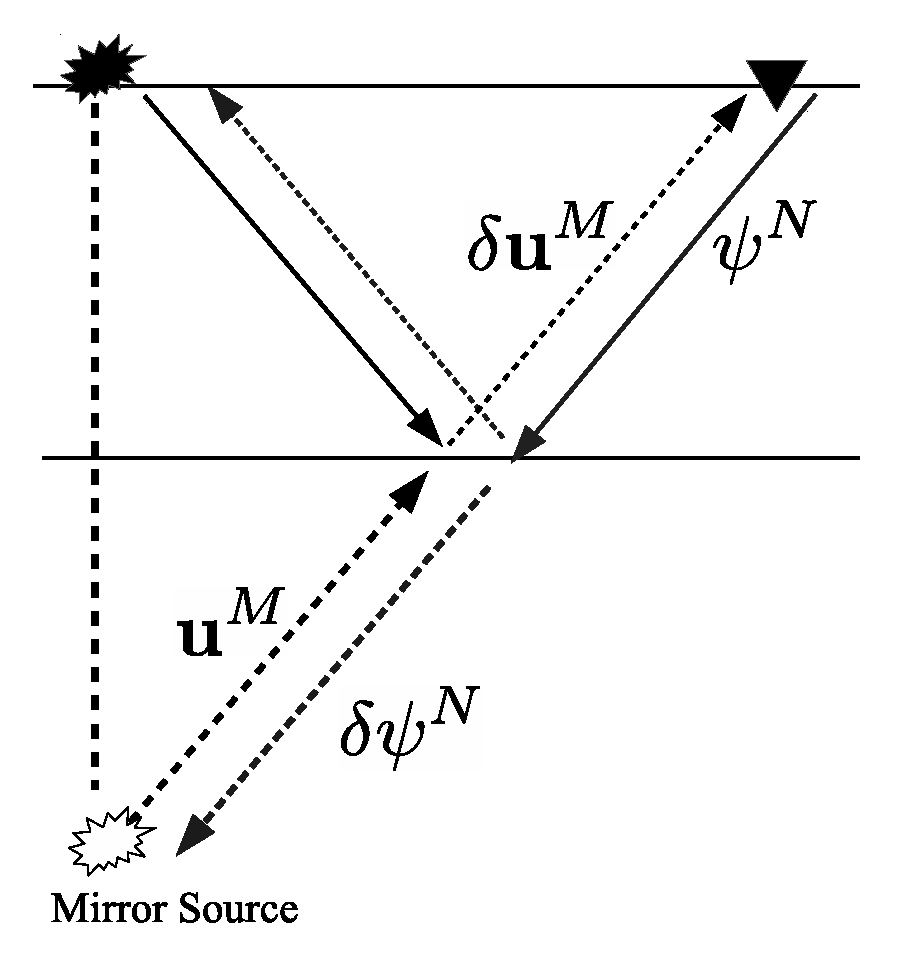
\includegraphics[width=0.5\textwidth]{Kernel/Combinations/K_MN.eps}}
   \caption{Schematic illustration of the reflection kernels $K^{MN}$. The
   cross-correlation can be regarded as the conventional FWI kernel between the mirror
   source and the receiver. The kernel can be a migration impulse or a
   transimission-type wavepath.}
   \label{fig:kernel_mirror_src}
\end{figure}
\begin{figure}
   \centering
   \subfigure[]{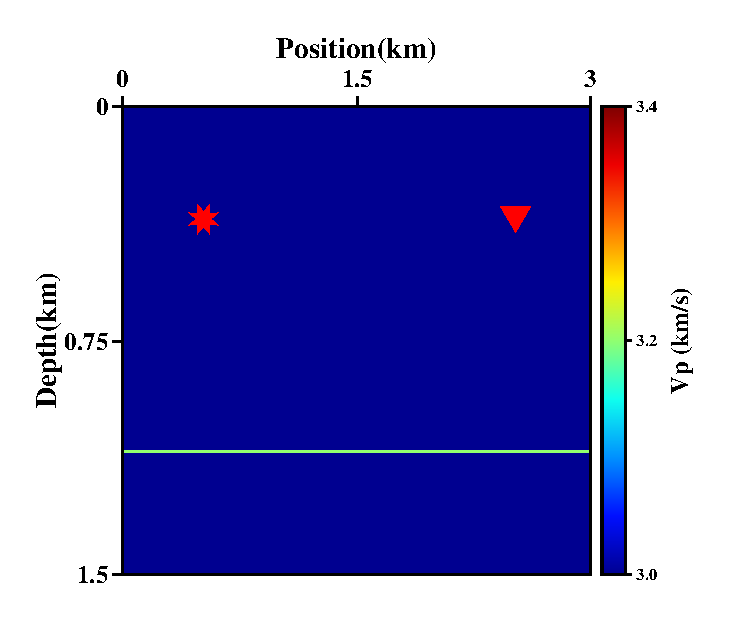
\includegraphics[width=0.45\textwidth]{Kernel/1vp.eps}}
   \subfigure[]{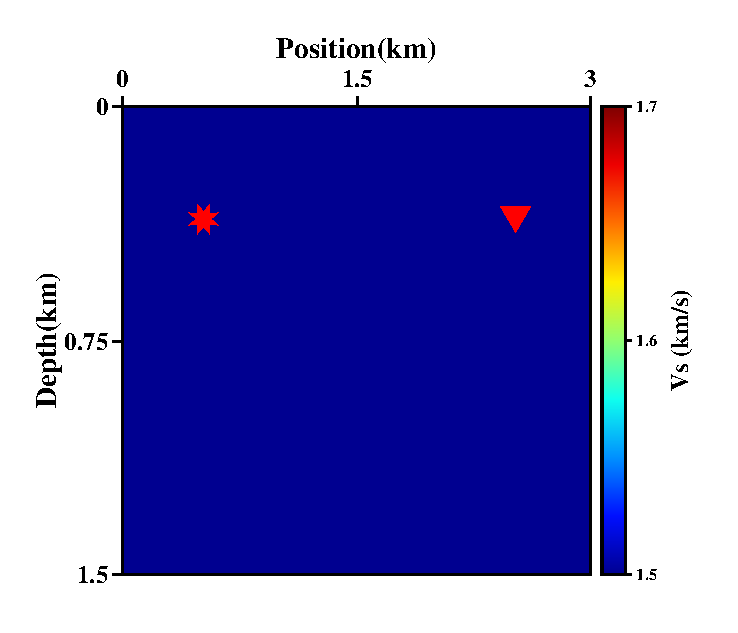
\includegraphics[width=0.45\textwidth]{Kernel/1vs.eps}}\\
   \subfigure[]{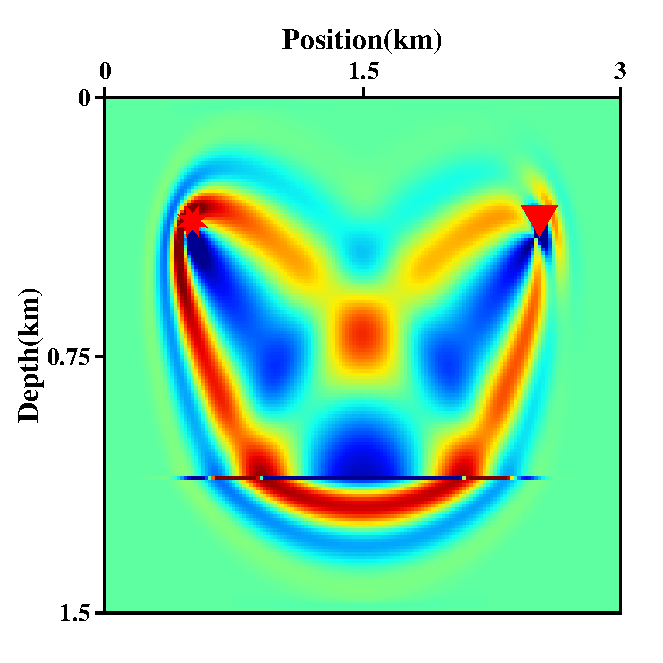
\includegraphics[width=0.45\textwidth]{Kernel/Vponlyvp.eps}}
   \subfigure[]{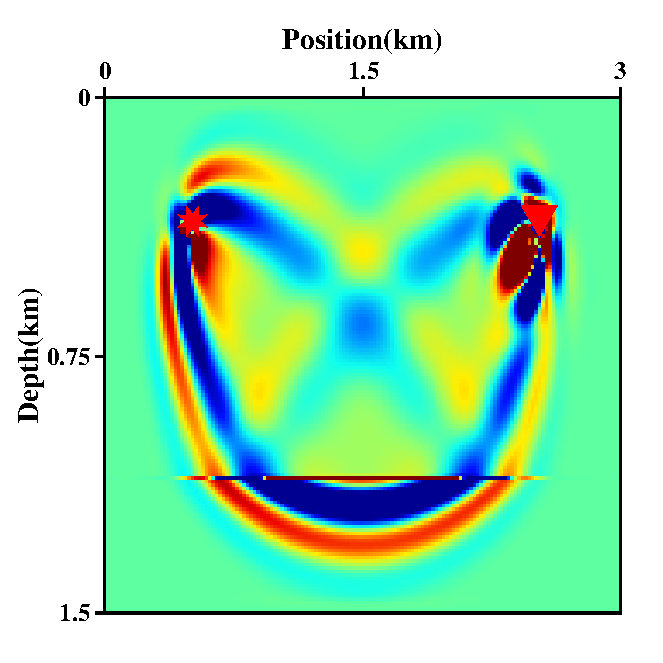
\includegraphics[width=0.45\textwidth]{Kernel/Vsonlyvp.eps}}\\
   \caption{Kernels with single reflector in $V_p$ model. (a) $V_p$ model, (b) $V_s$ model, (c) $K_{V_p}$, (d) $K_{V_s}$.}
   \label{fig:kernel1_vp}
\end{figure}

\begin{figure}
   \centering
   \subfigure[]{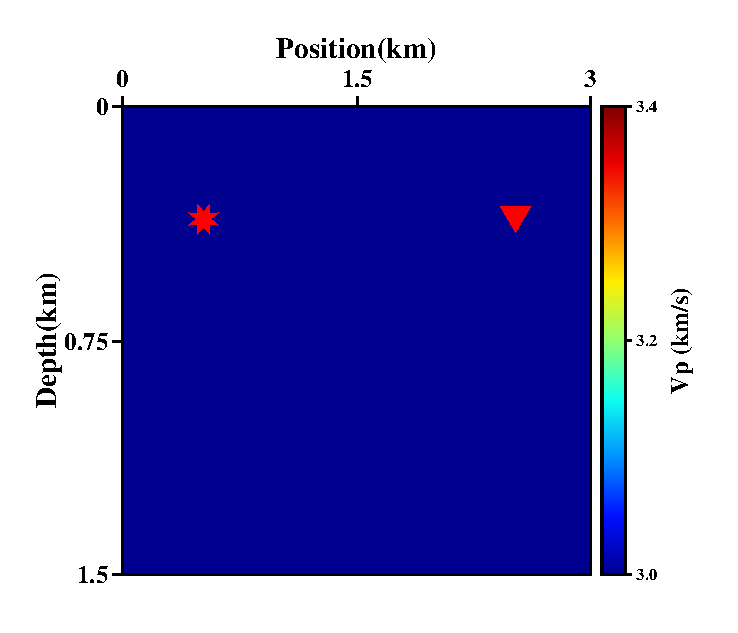
\includegraphics[width=0.450\textwidth]{Kernel/2vp.eps}}
   \subfigure[]{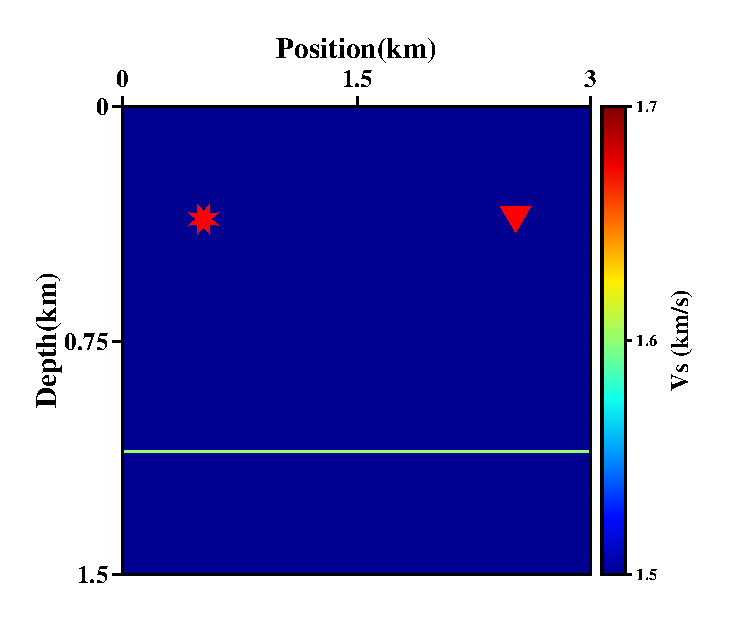
\includegraphics[width=0.450\textwidth]{Kernel/2vs.eps}}\\
   \subfigure[]{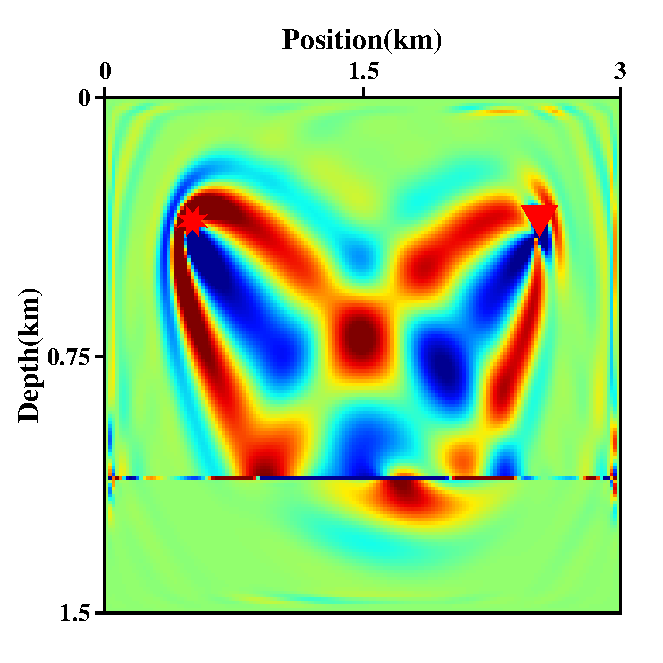
\includegraphics[width=0.450\textwidth]{Kernel/Vponlyvs.eps}}
   \subfigure[]{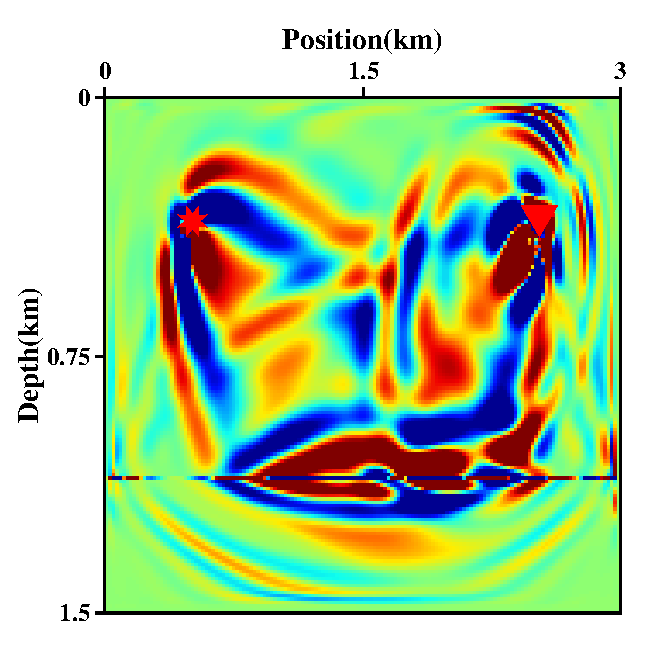
\includegraphics[width=0.450\textwidth]{Kernel/Vsonlyvs.eps}}\\
   \caption{Kernels with single reflector in $V_s$ model. (a) $V_p$ model, (b) $V_s$ model, (c) $K_{V_p}$, (d) $K_{V_s}$.}
   \label{fig:kernel2}
\end{figure}

\begin{figure}
   \centering
   \subfigure[]{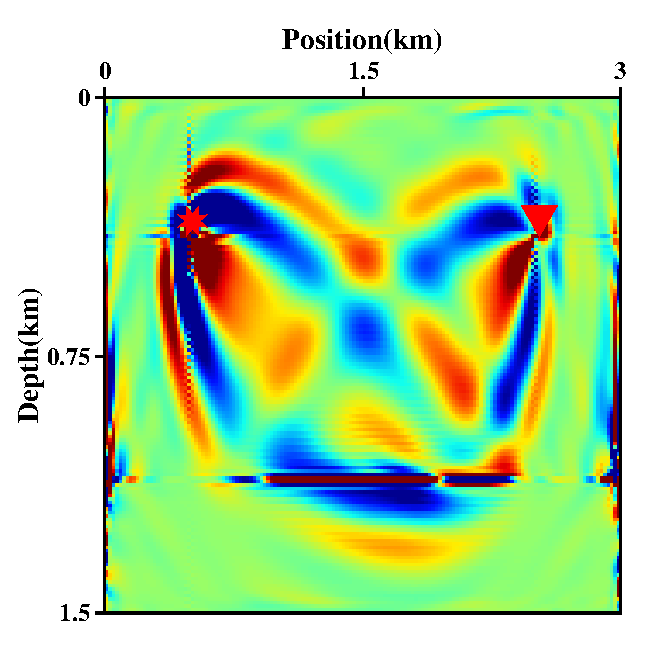
\includegraphics[width=0.450\textwidth]{Kernel/VsonlyvsPP.eps}}
   \subfigure[]{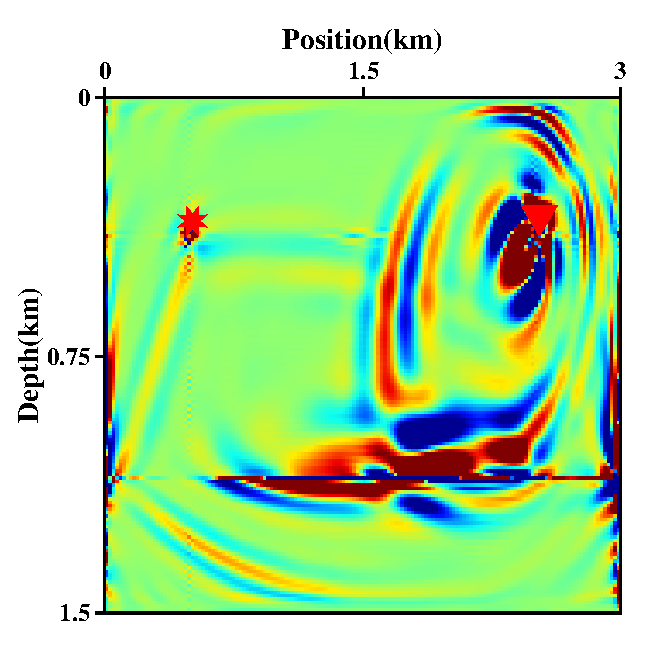
\includegraphics[width=0.450\textwidth]{Kernel/VsonlyvsPS.eps}}\\
   \subfigure[]{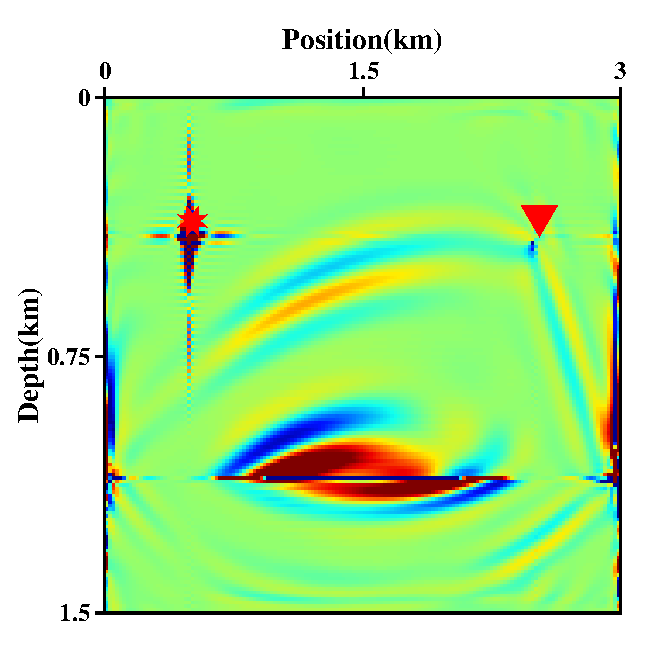
\includegraphics[width=0.450\textwidth]{Kernel/VsonlyvsSP.eps}}
   \subfigure[]{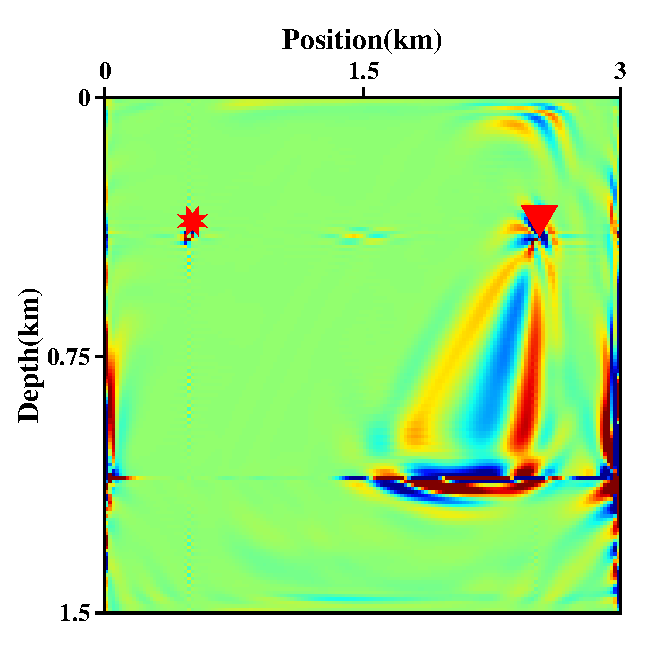
\includegraphics[width=0.450\textwidth]{Kernel/VsonlyvsSS.eps}}
   \caption{Four components of $K_{V_s}$. Here we only decompose the subsurface wavefields as in
   eq. \eqref{eq:decompkernel} but do not separate the data for injection. 
   (a) $K_{V_s}^{PP}$, (b) $K_{V_s}^{PS}$, (c) $K_{V_s}^{SP}$, (d) $K_{V_s}^{SS}$.}
   \label{fig:kernel2_vs_decomp}
\end{figure}
\begin{figure}
   \centering
   {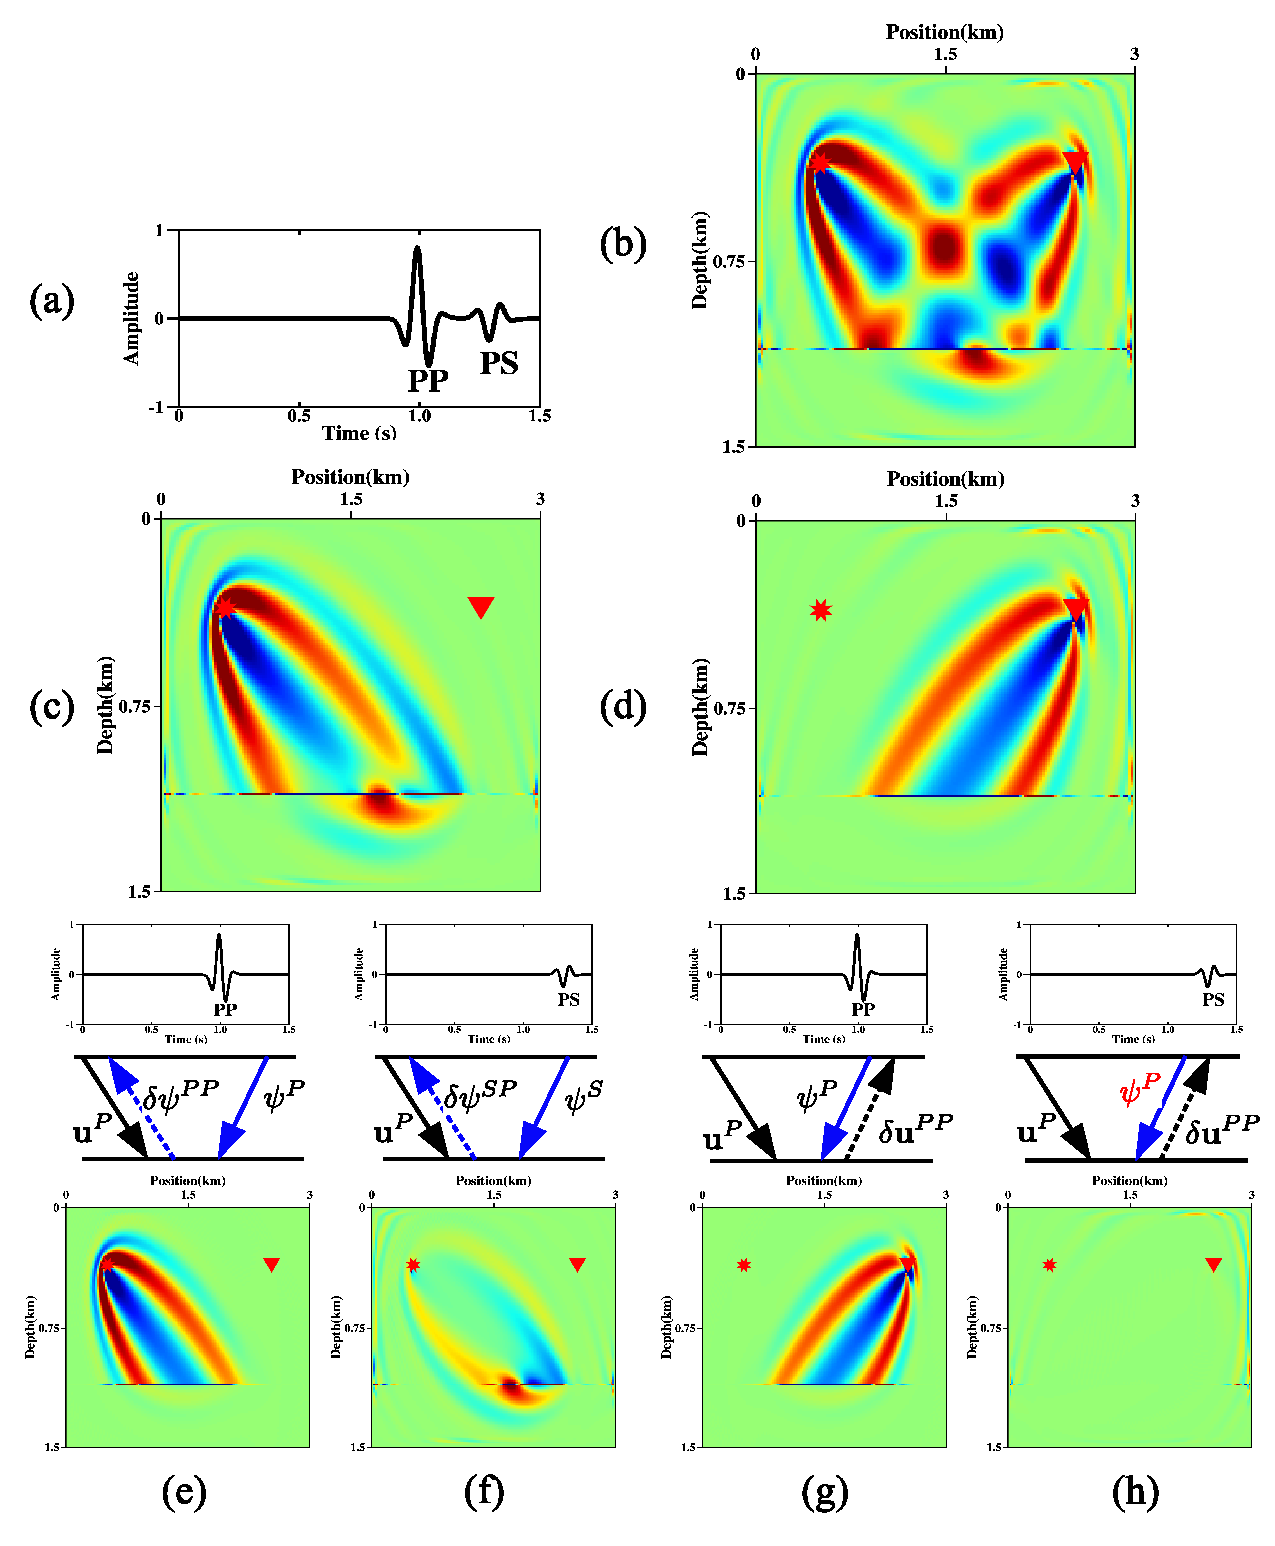
\includegraphics[width=0.8\textwidth]{Kernel/Combinations/K_vp.eps}}
   \caption{
   Further decomposition of $K_{V_p}$ for the second test by injecting the PP
   and PS event separately as adjoint source and decomposing the wavefields with different manners. 
   (a) Original adjoint source
   for back-propagation, (b) $K_{V_p}$, (c) Source side of $K_{V_p}$, (d)
   Receiver side of $K_{V_p}$. (e)-(h): The first line denotes the adjoint source. 
   The second line denotes the manner of mode decomposition. The last line
   denote the corresponding kernel. Note that, when injecting PS data, a
   non-physical SP conversion (red) is generated
%   So that there will be a migration impulse
   in panel (h)}
   \label{fig:kernel_vp_decomp}
\end{figure}
\begin{figure}
   \centering
   {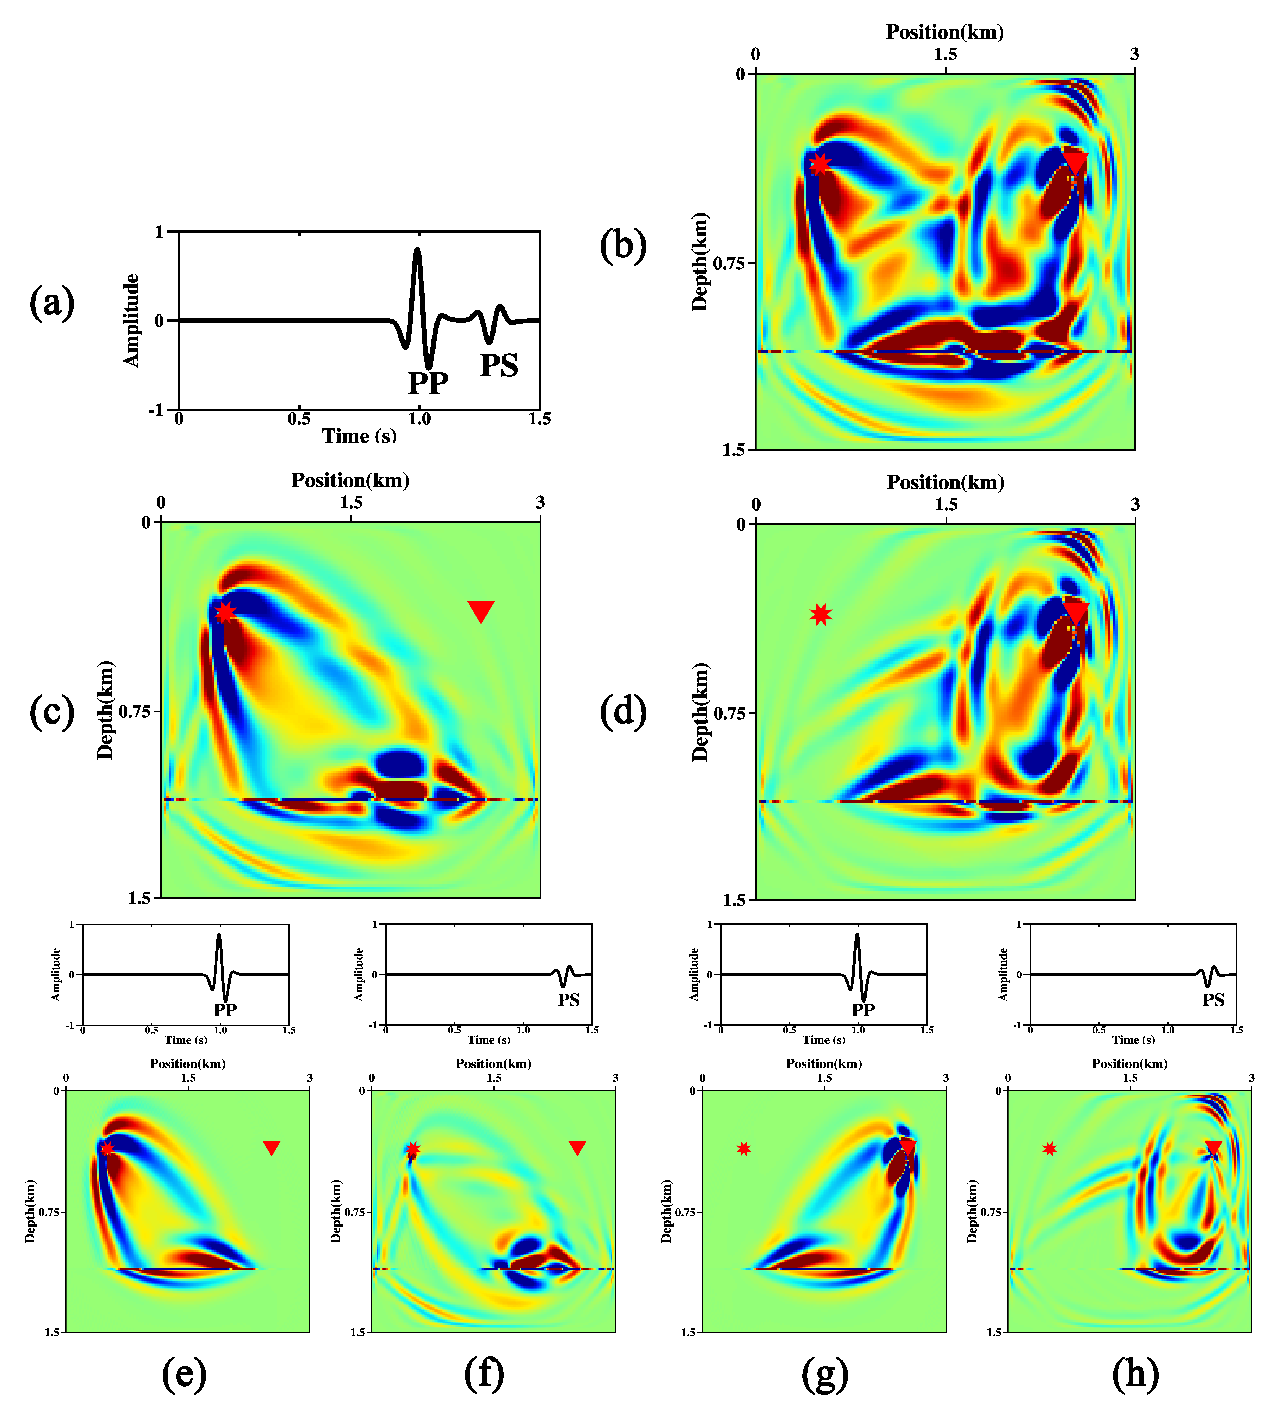
\includegraphics[width=1.0\textwidth]{Kernel/Combinations/K_vs1.eps}}
   \caption{
   Further decomposition of $K_{V_s}$ for the second test. Here we only separate PP and PS data
   for injection. (a): Original adjoint source
   , (b) $K_{V_s}$, (c) Source term of $K_{V_s}$, (d)
   Receiver term of $K_{V_s}$. (e)-(h): The first line denotes the adjoint source for
   injection. The second line denotes the decomposed kernels when separately
   injecting PP and PS data. 
   }
   \label{fig:kernel_vs_decomp}
\end{figure}
\clearpage
\begin{figure}
   \centering
   {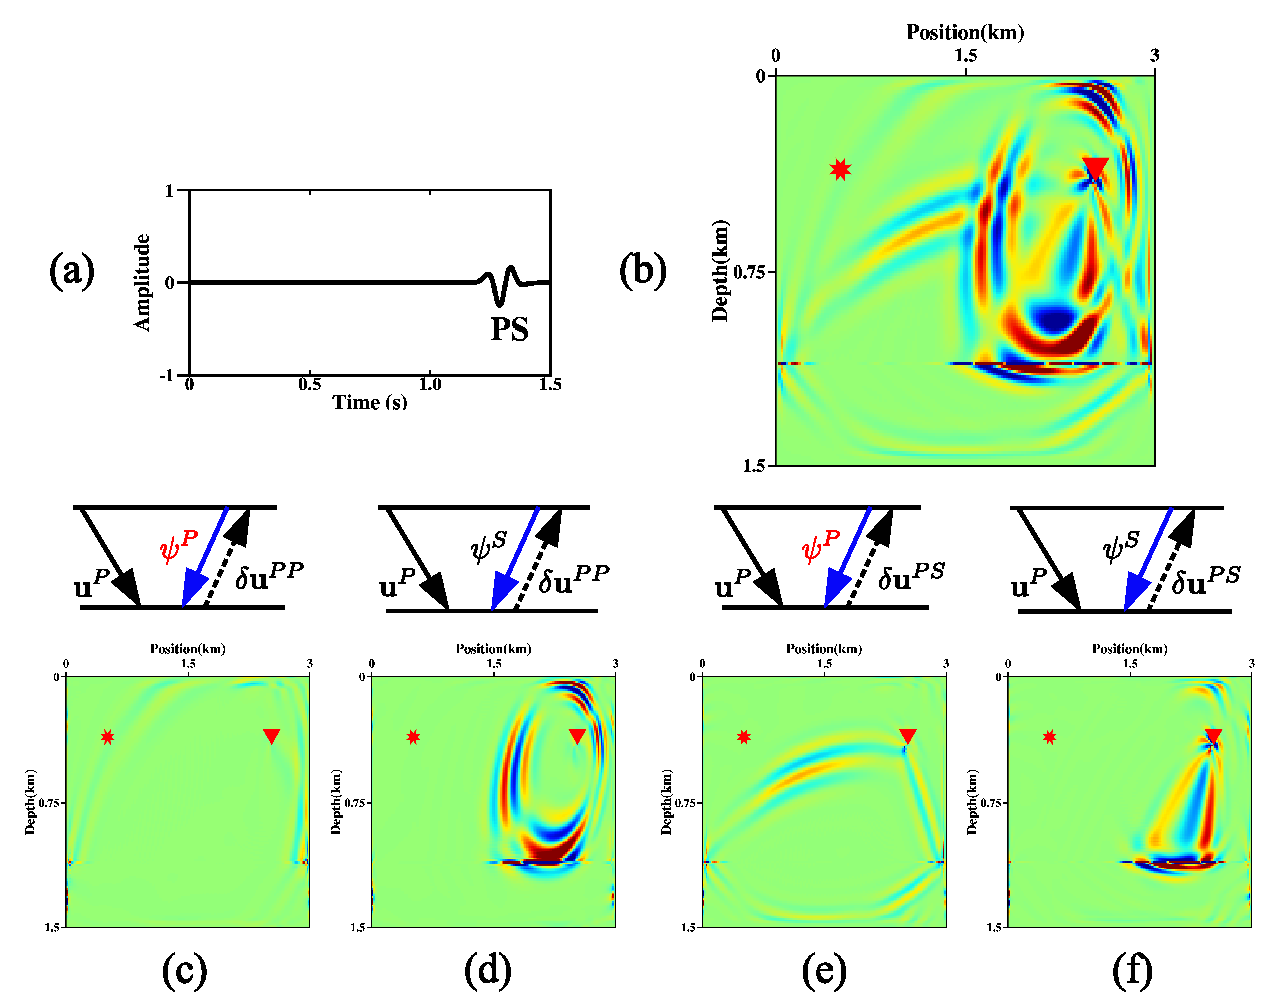
\includegraphics[width=1.0\textwidth]{Kernel/Combinations/K_vs_recPS.eps}}
   \caption{Further decomposed components of Fig \ref{fig:kernel_vs_decomp}h using spatial wave mode
   decomposition when only injecting PS data. (a) The adjoint source
   for injection, (b) Receiver term of $K_{V_s}$ using (a) as adjoint source, (c)-(f) 
   The first line denotes the manner and wavefield type for cross-correlation.
   The second line denotes the corresponding kernels.
   The $\psi^P$ in red denotes the non-physical conversion when injecting PS data.
   }
   \label{fig:kernel_vs_recPS}
\end{figure}

\clearpage

\begin{figure}
   \centering
   \subfigure[]{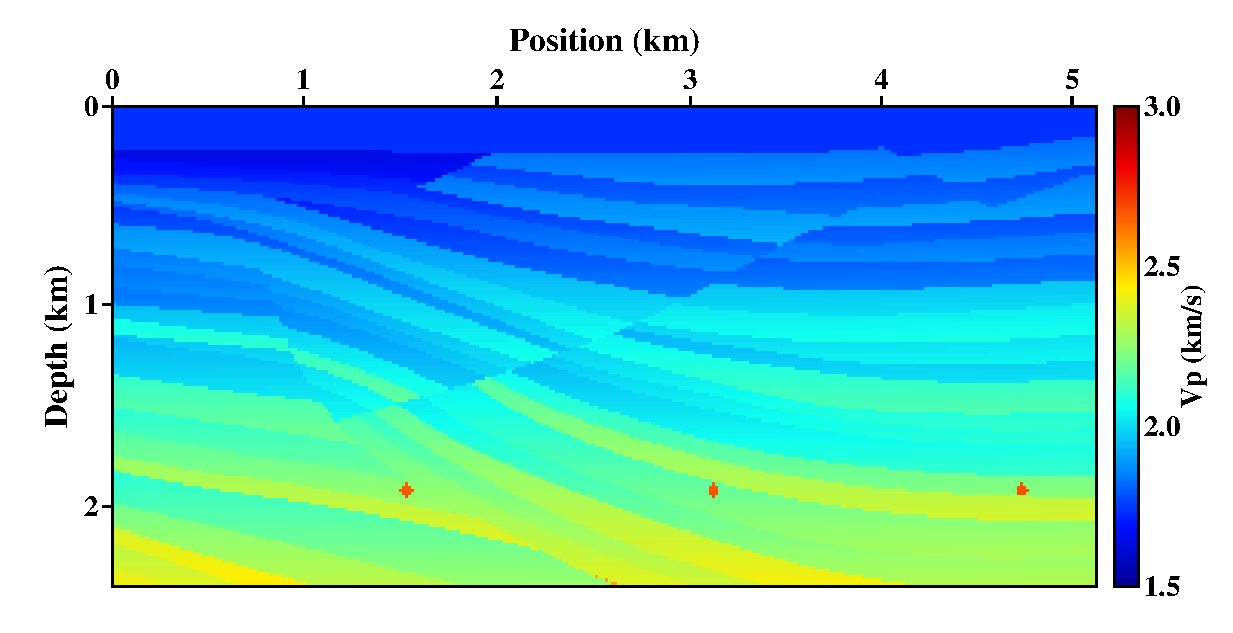
\includegraphics[width=0.45\textwidth]{sigbee2_new/Fig/Truevp.eps}}
   \subfigure[]{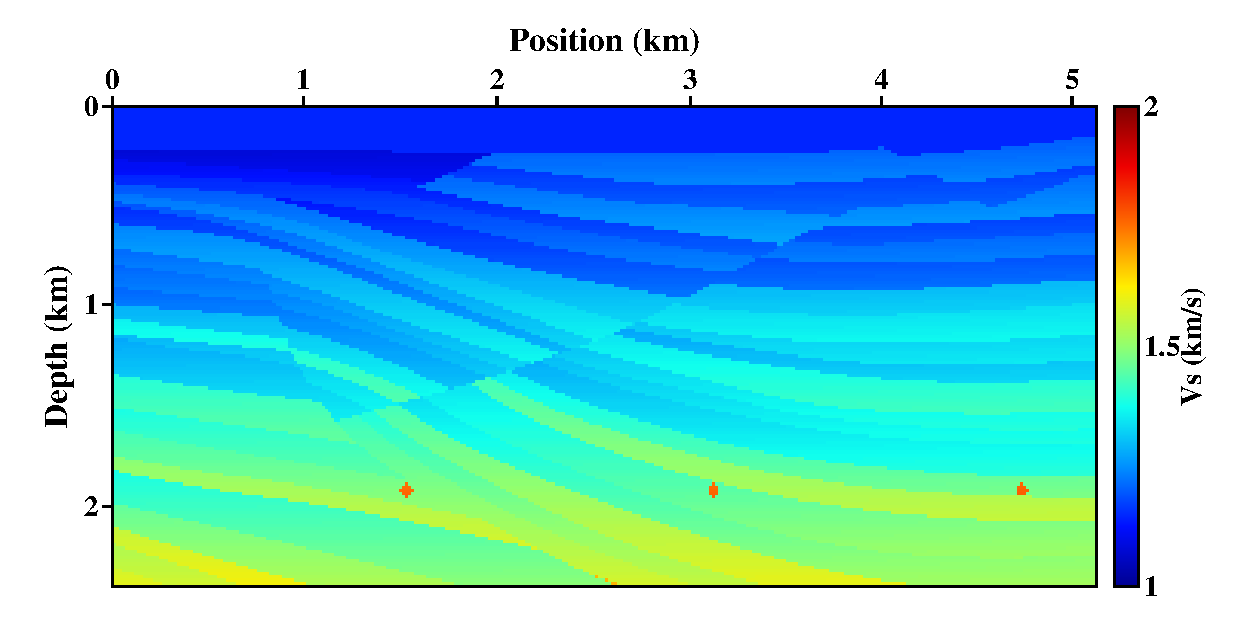
\includegraphics[width=0.45\textwidth]{sigbee2_new/Fig/Truevs.eps}}\\
   \subfigure[]{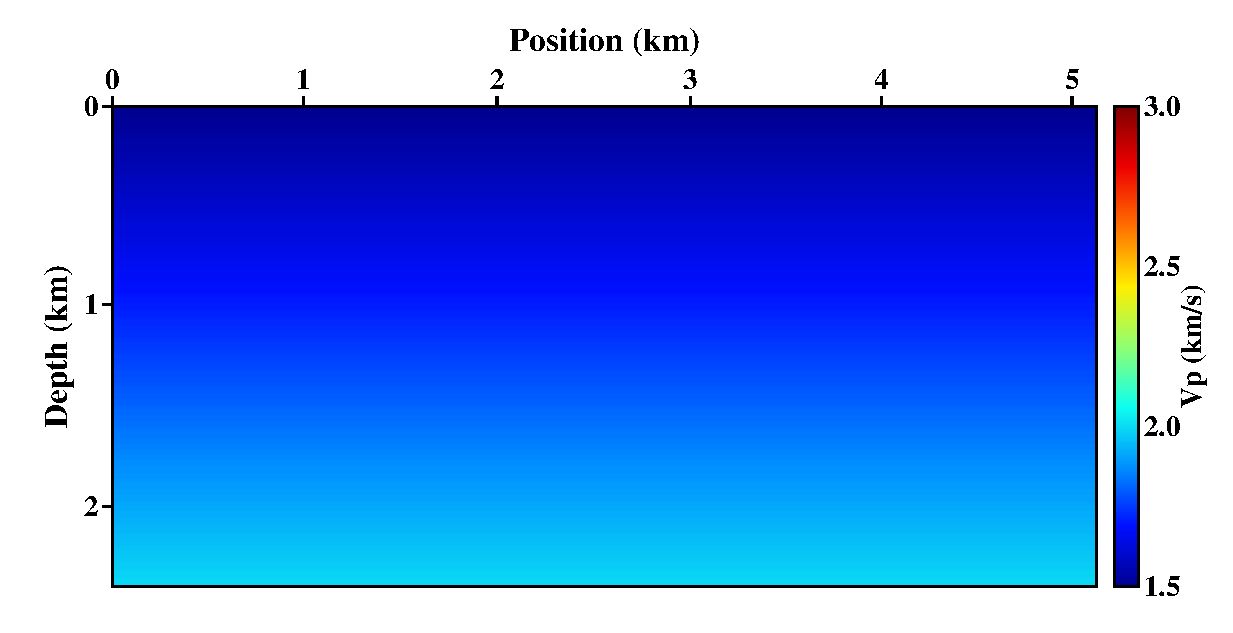
\includegraphics[width=0.45\textwidth]{sigbee2_new/Fig/Initvp.eps}}
   \subfigure[]{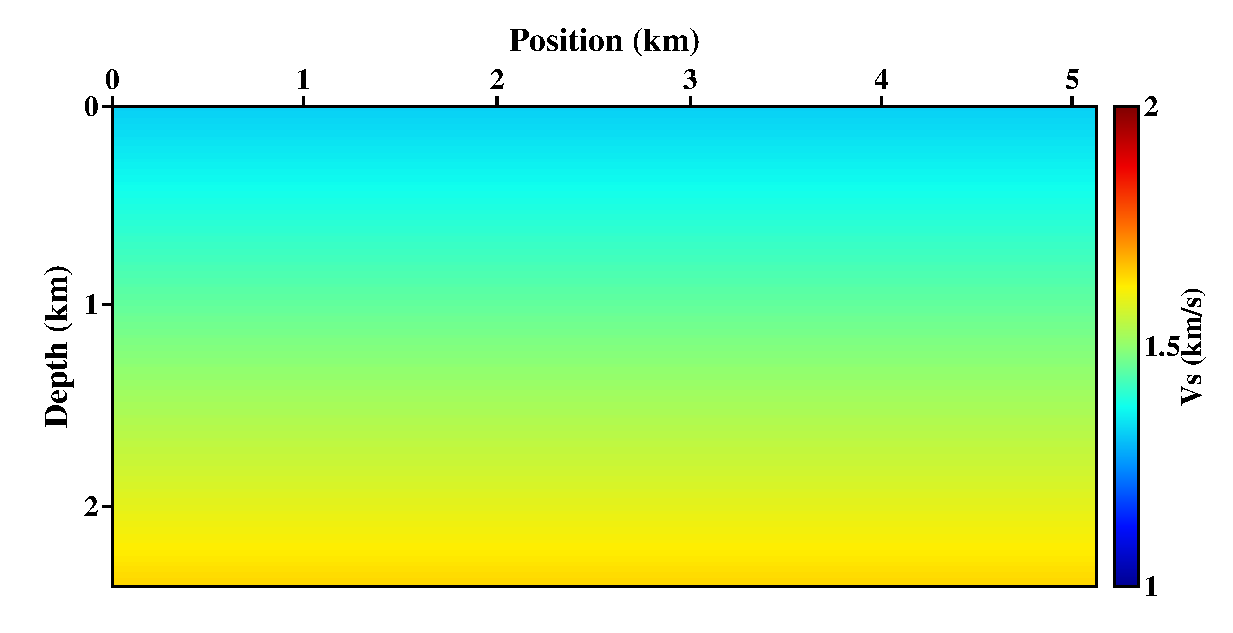
\includegraphics[width=0.45\textwidth]{sigbee2_new/Fig/Initvs.eps}}
   \caption{Sigbee2A model example. On the top are true models of 
   $V_p$ (a) and $V_s$ (b). On the bottom are initial models of $V_p$ (c) and $V_s$
   (d) linearly increasing with depth. }
   \label{fig:TrueAndInitial}
\end{figure}
\clearpage

\begin{figure}
   \centering
   \subfigure[]{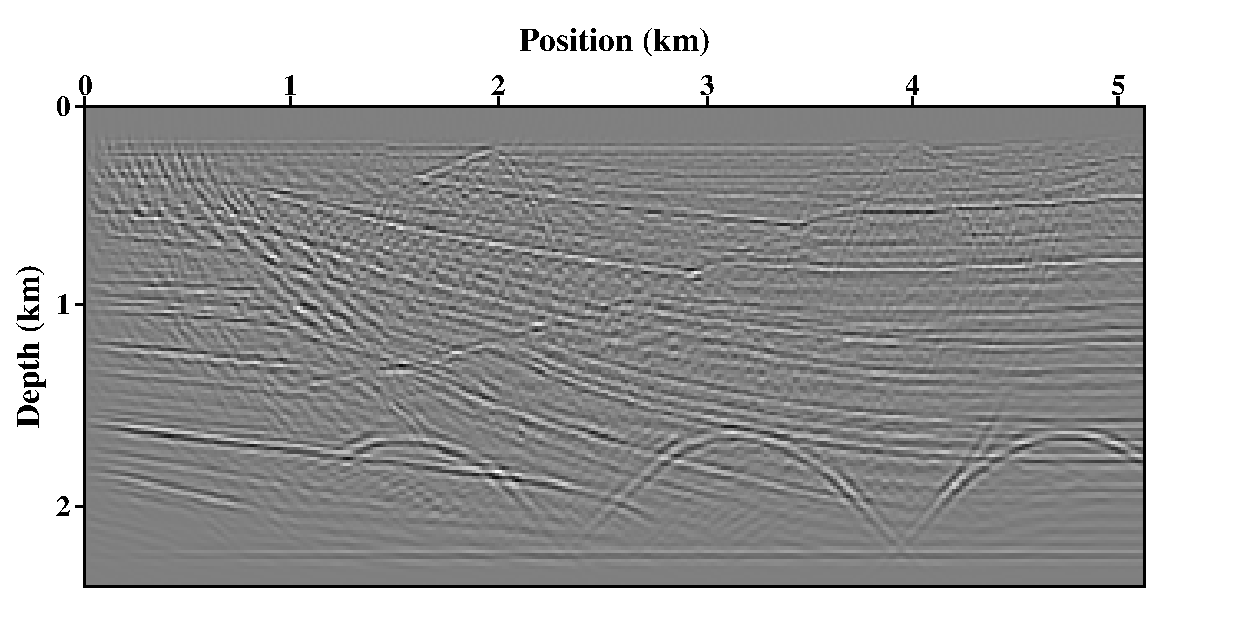
\includegraphics[width=0.45\textwidth]{sigbee2_new/Fig/imageInitialvp.eps}}
   \subfigure[]{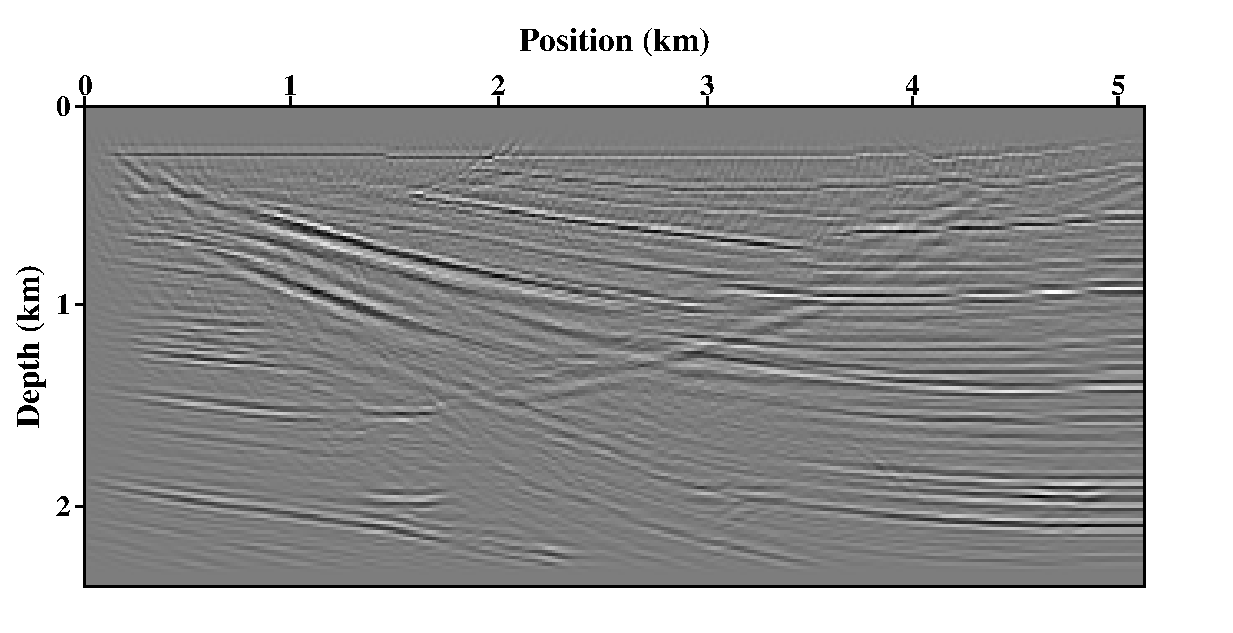
\includegraphics[width=0.45\textwidth]{sigbee2_new/Fig/imageInitialvs.eps}}\\
   \subfigure[]{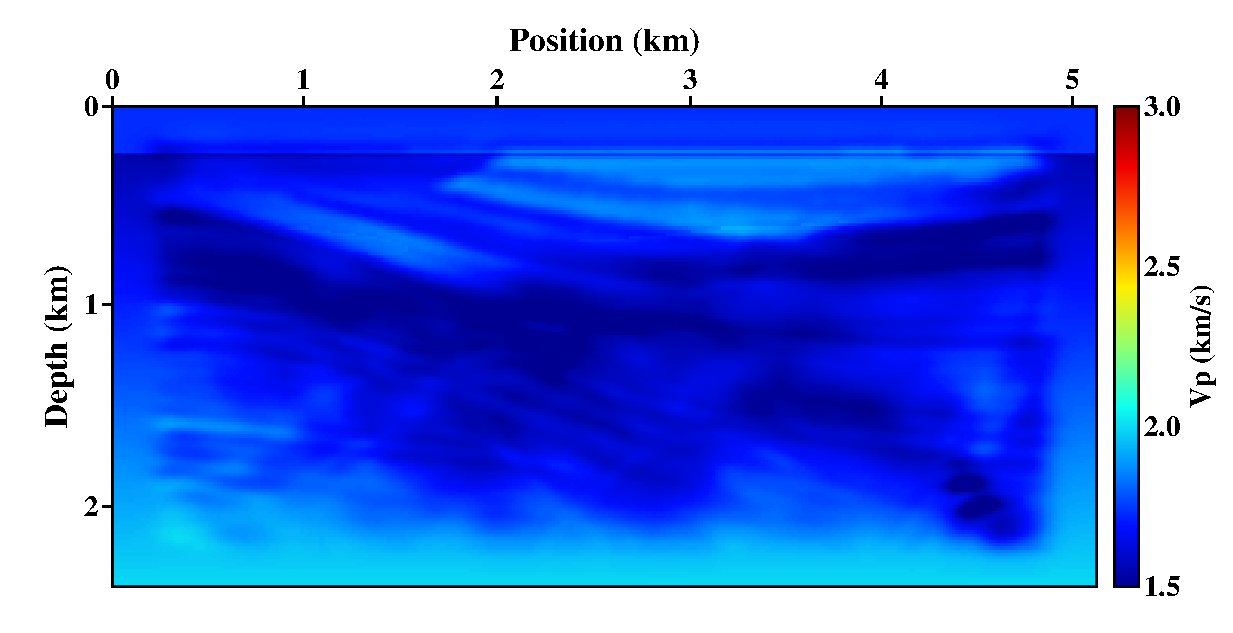
\includegraphics[width=0.45\textwidth]{sigbee2_new/Fig/badinitvp.eps}}
   \subfigure[]{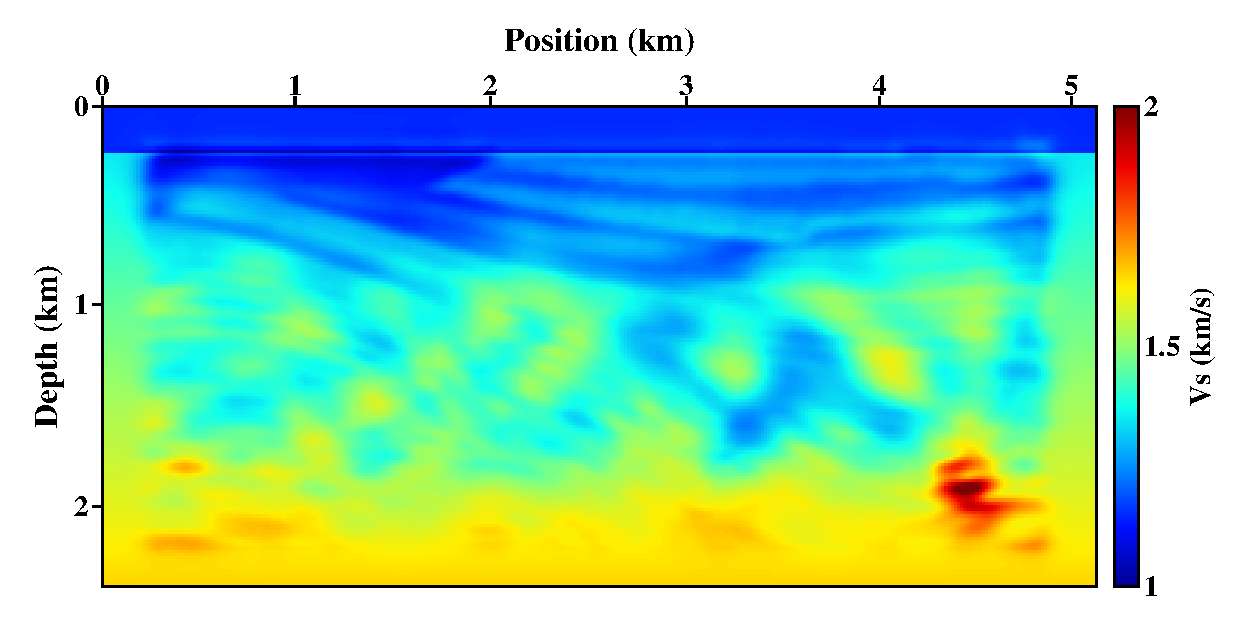
\includegraphics[width=0.45\textwidth]{sigbee2_new/Fig/badinitvs.eps}}\\
   \caption{The results of ERTM and EFWI using initial model: (a) and (b) are PP and
   PS image of ERTM with near offset data, (c) and (d) are inverted $V_p$ and $V_s$
   with EFWI.}
   \label{fig:Results_init}
\end{figure}
\clearpage
\begin{figure}
   \centering
   \subfigure[]{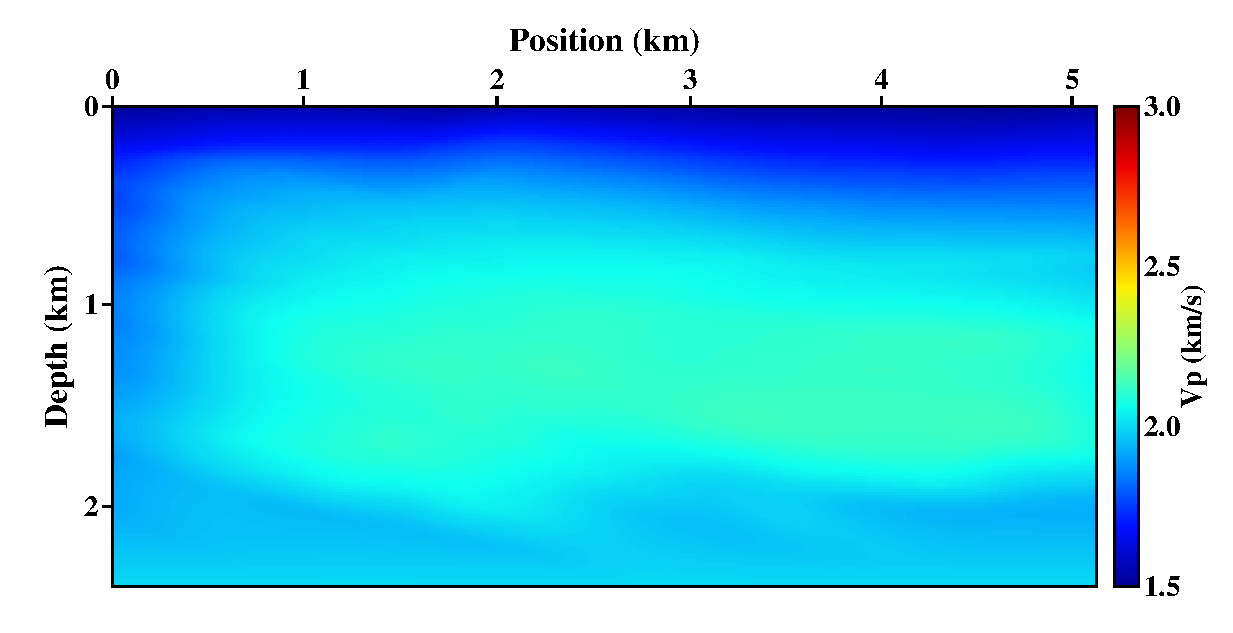
\includegraphics[width=0.45\textwidth]{sigbee2_new/Fig/RTIvp.eps}}
   \subfigure[]{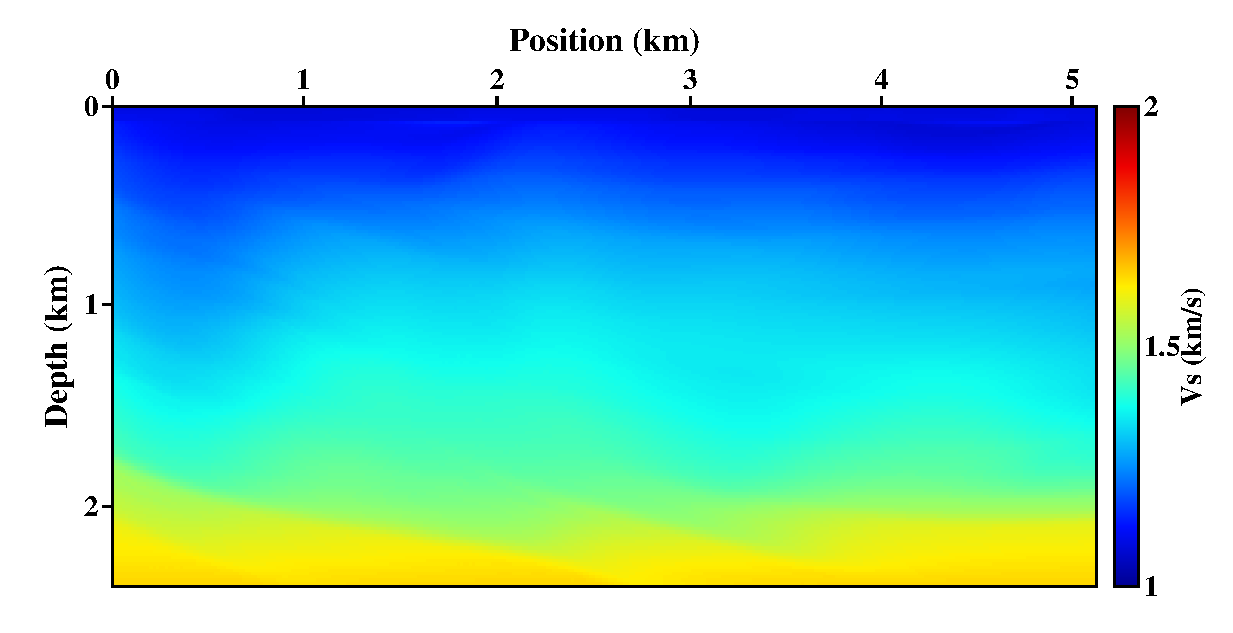
\includegraphics[width=0.45\textwidth]{sigbee2_new/Fig/RTIvs.eps}}\\
   \caption{Inverted results of ERTI: (a) $V_p$, (b) $V_s$.}
   \label{fig:InvertedModel_ERTI}
\end{figure}
\clearpage
\begin{figure}
   \centering
   \subfigure[]{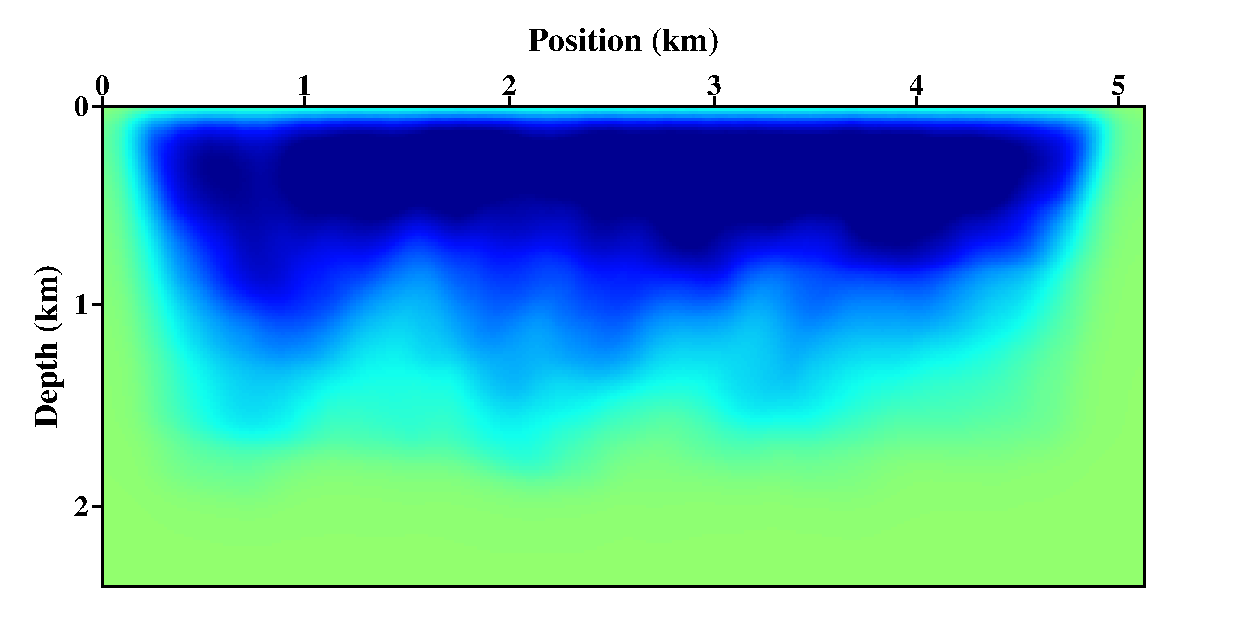
\includegraphics[width=0.45\textwidth]{sigbee2/NoLSF_Gra_vp.eps}}
   \subfigure[]{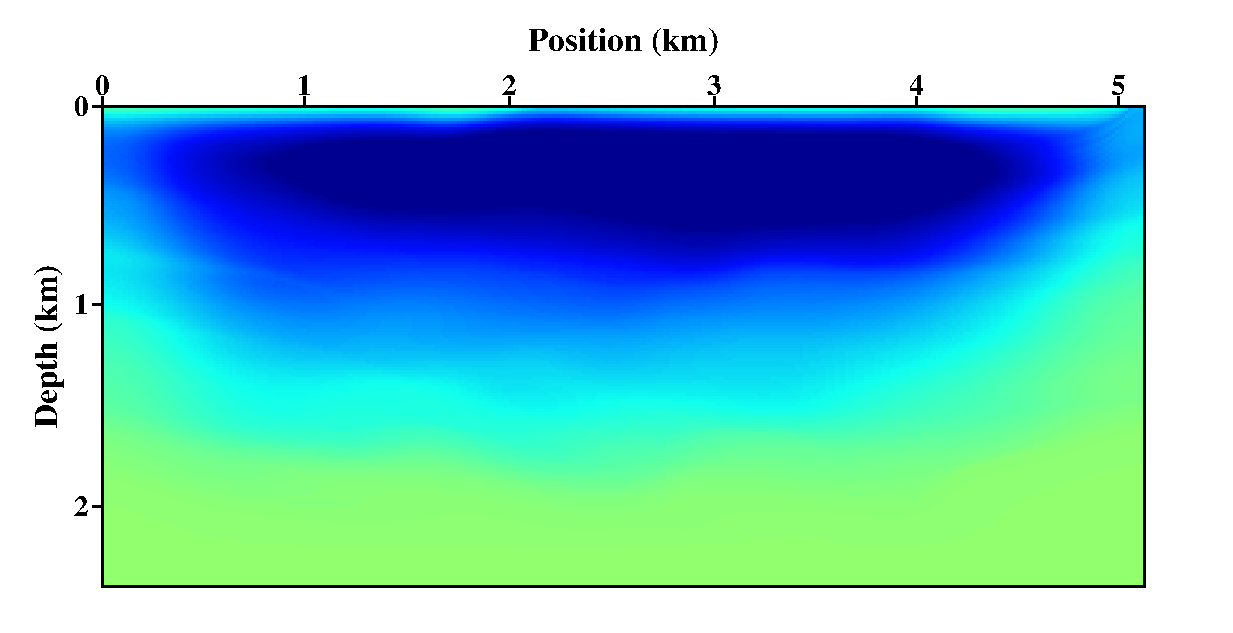
\includegraphics[width=0.45\textwidth]{sigbee2/LSF_Gra_vp.eps}}
 %  \subfigure[]{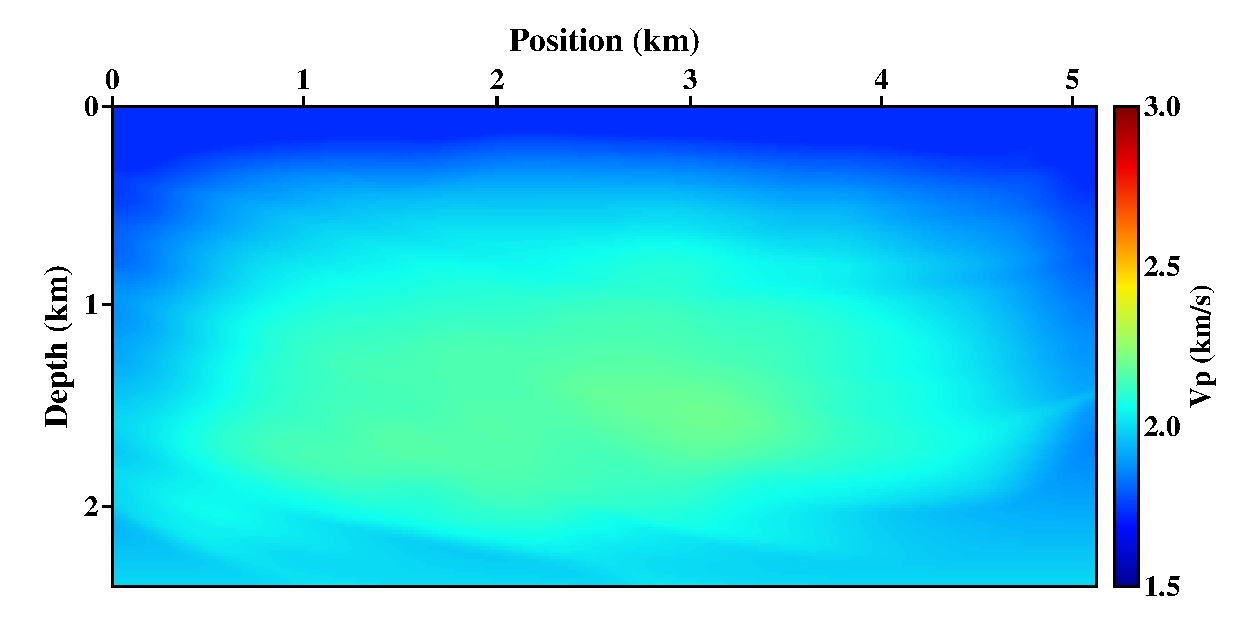
\includegraphics[width=0.5\textwidth]{sigbee2/Fig/newinit3vp.eps}}
 %  \subfigure[]{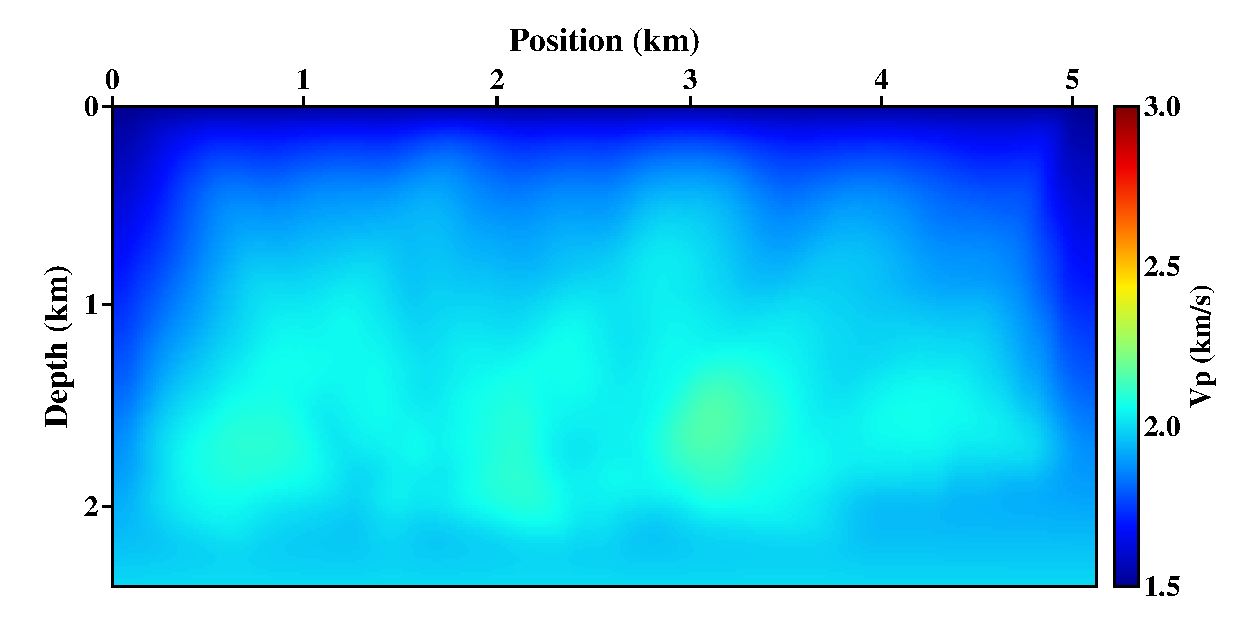
\includegraphics[width=0.5\textwidth]{sigbee2/NoLSF_vp.eps}}\\
   \caption{The comparison of gradients without (a) and   with (b) 
   the structure-oriented constrain. }
   \label{fig:LSF_comparison}
\end{figure}
\clearpage
\begin{figure}
   \centering
   \subfigure[]{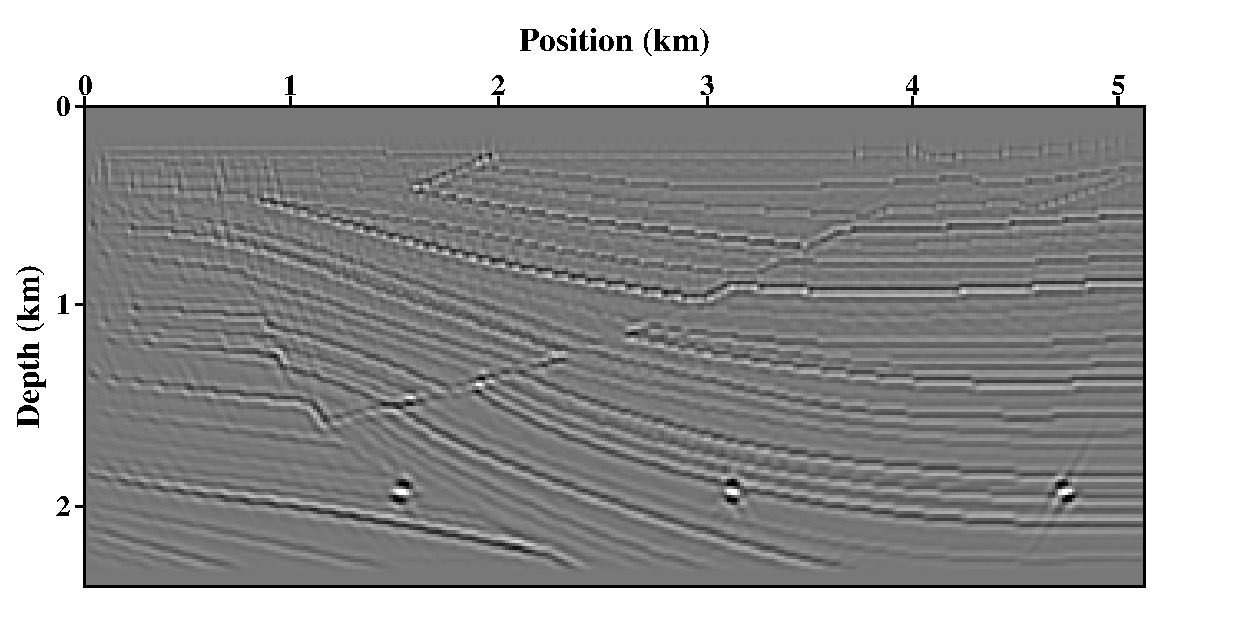
\includegraphics[width=0.45\textwidth]{sigbee2_new/Fig/imageTRUEvp.eps}}
   \subfigure[]{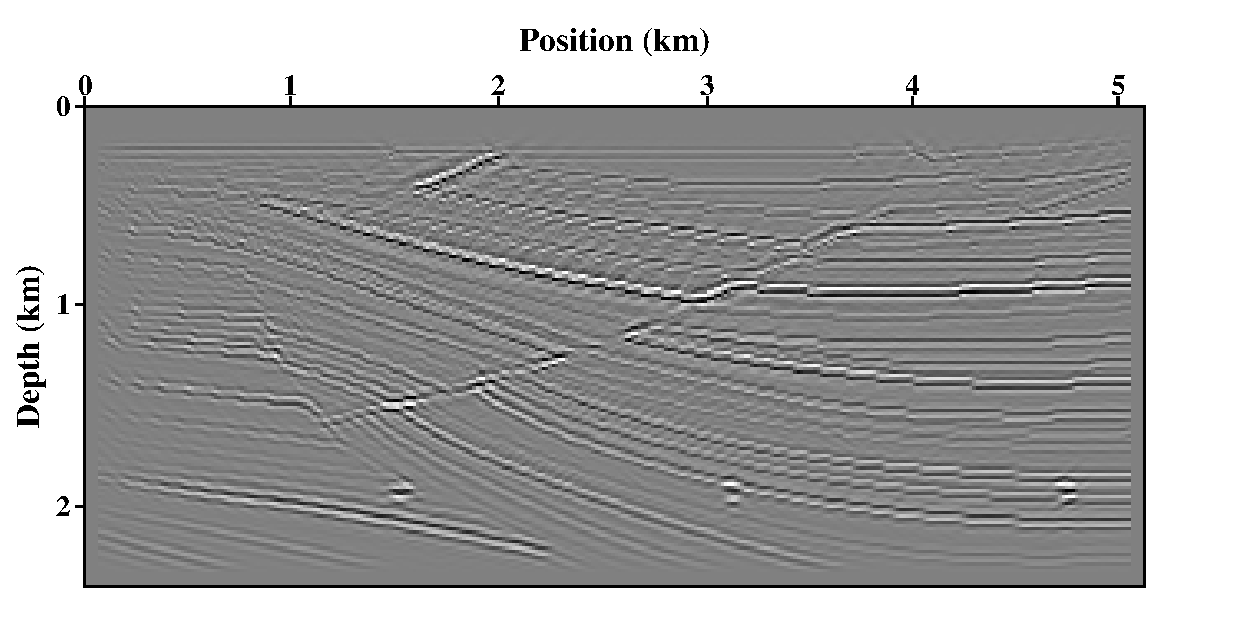
\includegraphics[width=0.45\textwidth]{sigbee2_new/Fig/imageTRUEvs.eps}}\\
   \subfigure[]{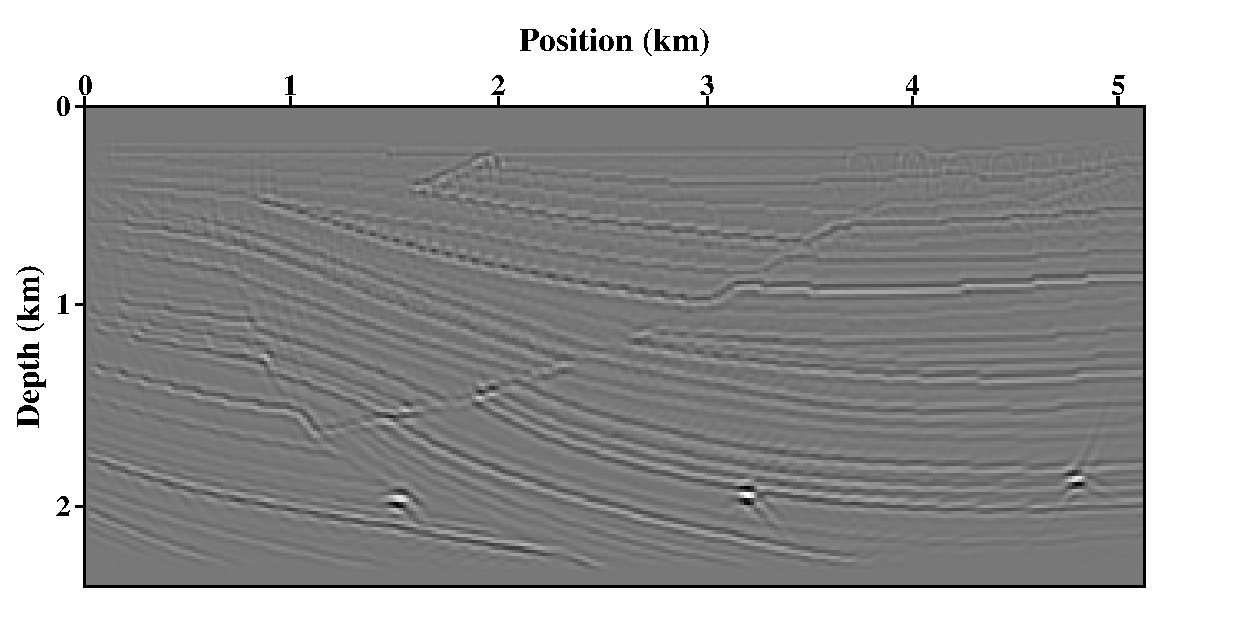
\includegraphics[width=0.45\textwidth]{sigbee2_new/Fig/imageRTIvp.eps}}
   \subfigure[]{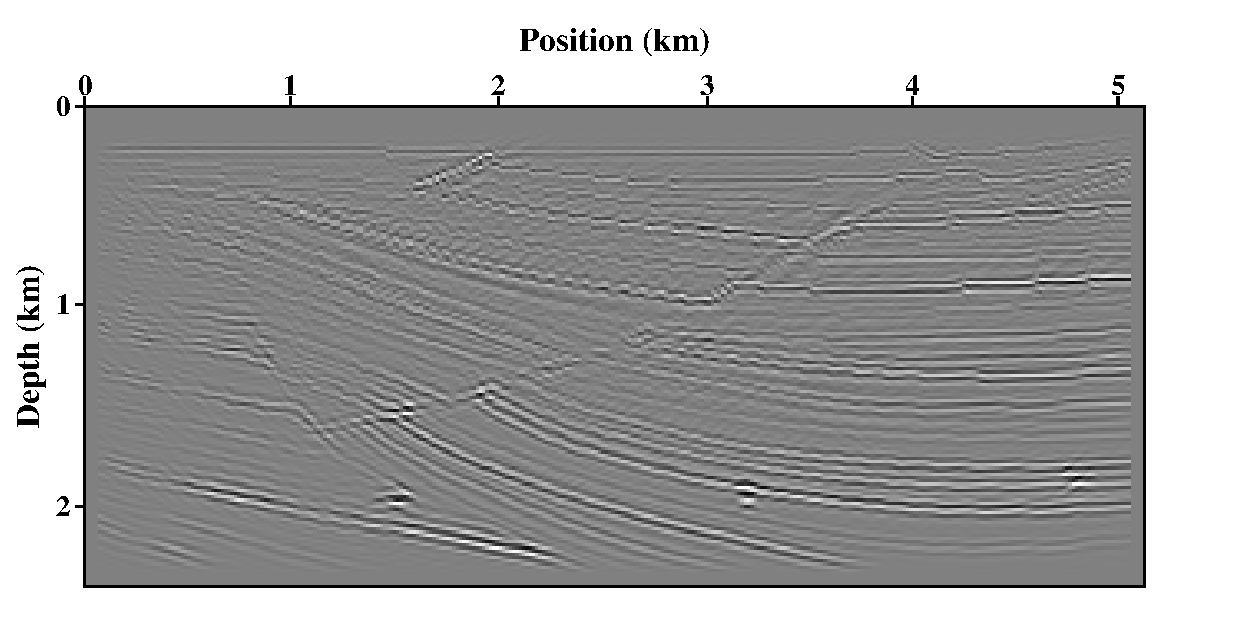
\includegraphics[width=0.45\textwidth]{sigbee2_new/Fig/imageRTIvs.eps}}
   \caption{ERTM results using the true model (a, b) and
   inverted model (c, d). (a) and (c) are the PP image;(b) and (d) are the PS
   image}
   \label{fig:ERTM_comparison}
\end{figure}
\begin{figure}
   \centering
   \subfigure[]{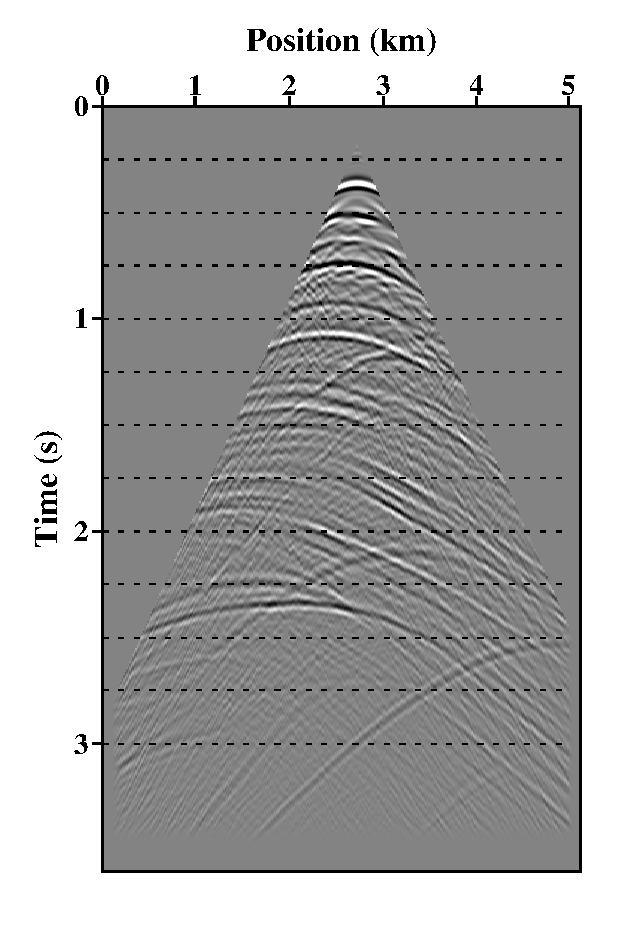
\includegraphics[width=0.30\textwidth]{sigbee2/Fig/DataPP_true.eps}}
   \subfigure[]{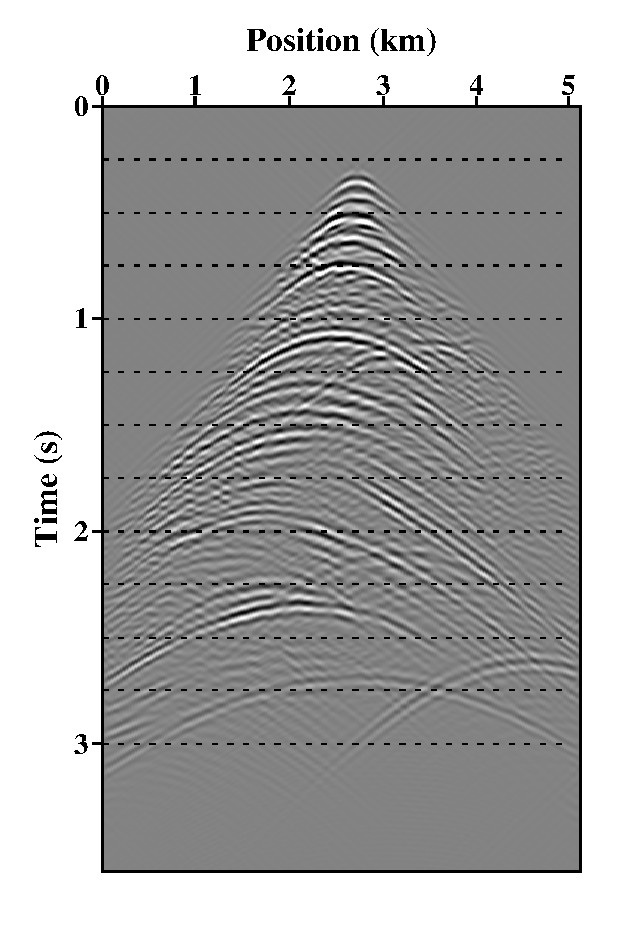
\includegraphics[width=0.30\textwidth]{sigbee2/Fig/DataPP_init.eps}}
   \subfigure[]{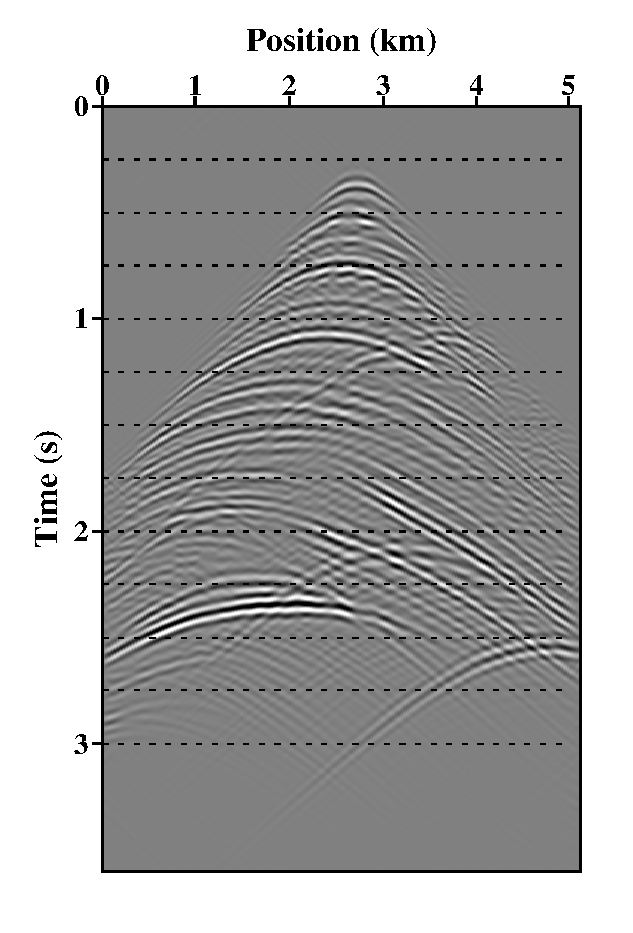
\includegraphics[width=0.30\textwidth]{sigbee2/Fig/DataPP_werti.eps}}\\
   \subfigure[]{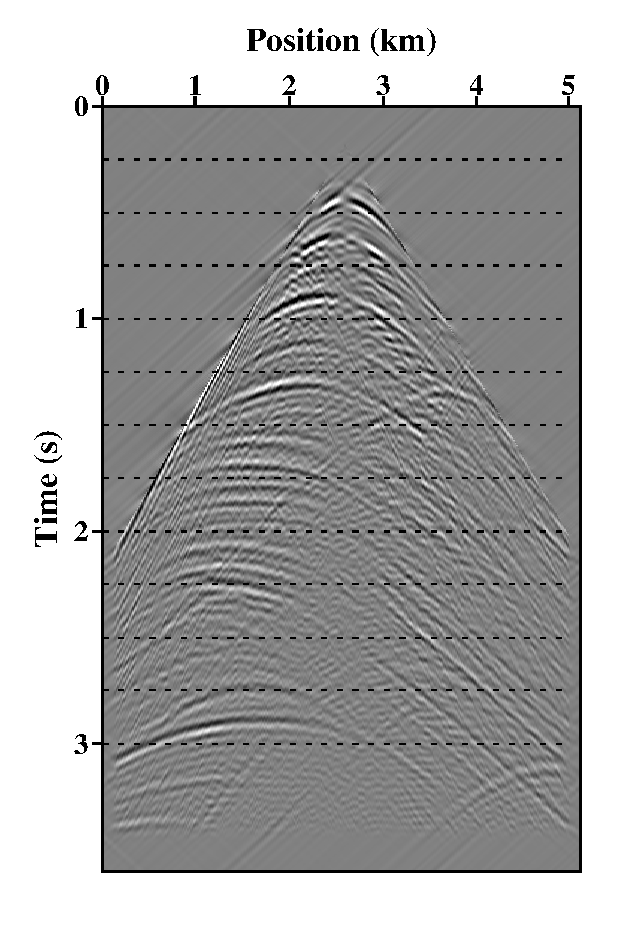
\includegraphics[width=0.30\textwidth]{sigbee2/Fig/DataPS_true.eps}}
   \subfigure[]{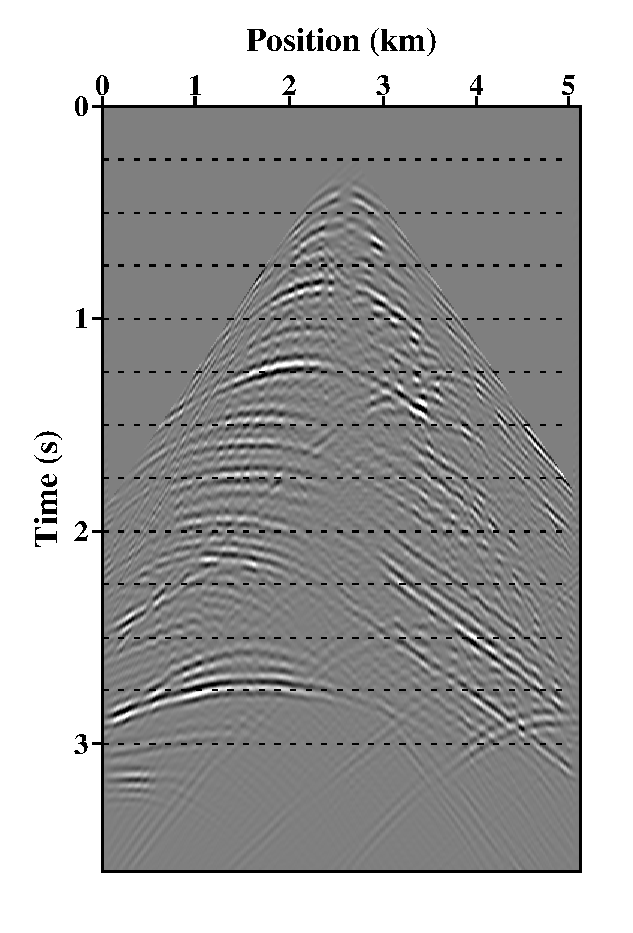
\includegraphics[width=0.30\textwidth]{sigbee2/Fig/DataPS_init.eps}}
   \subfigure[]{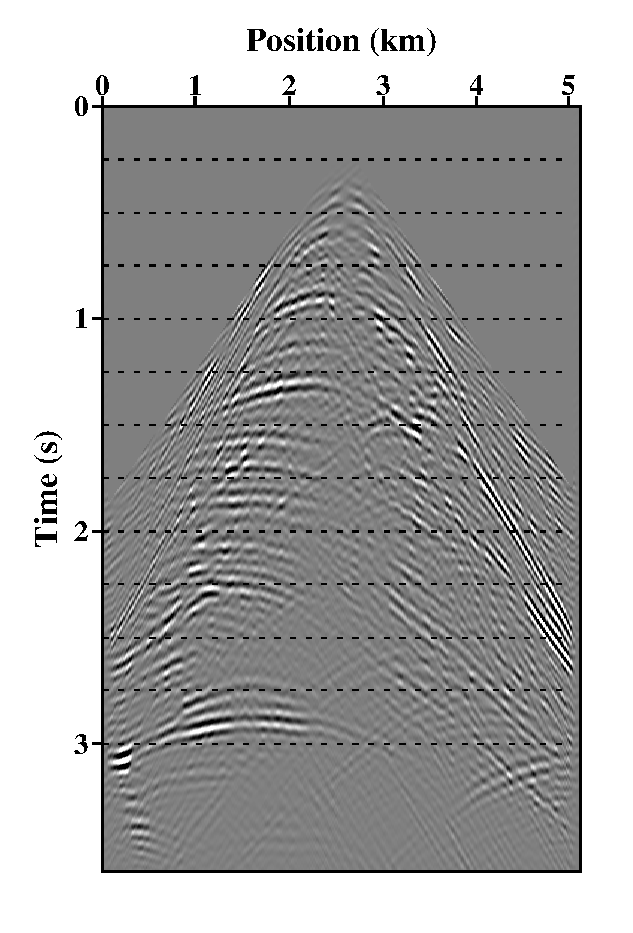
\includegraphics[width=0.30\textwidth]{sigbee2/Fig/DataPS_werti.eps}}
   \caption{Comparison of the observed and the demigrated reflection data using
   initial model and the inverted model. The first row are the separated PP
   reflection, while the second row are the separated PS reflection. 
   The left, middle and right column are the observed reflection data, the
   demigrated reflection data with initial model
   and the demigrated data with inverted model, respectively. }
   \label{fig:Data_comparison}
\end{figure}

\clearpage
\begin{figure}
   \centering
   \subfigure[]{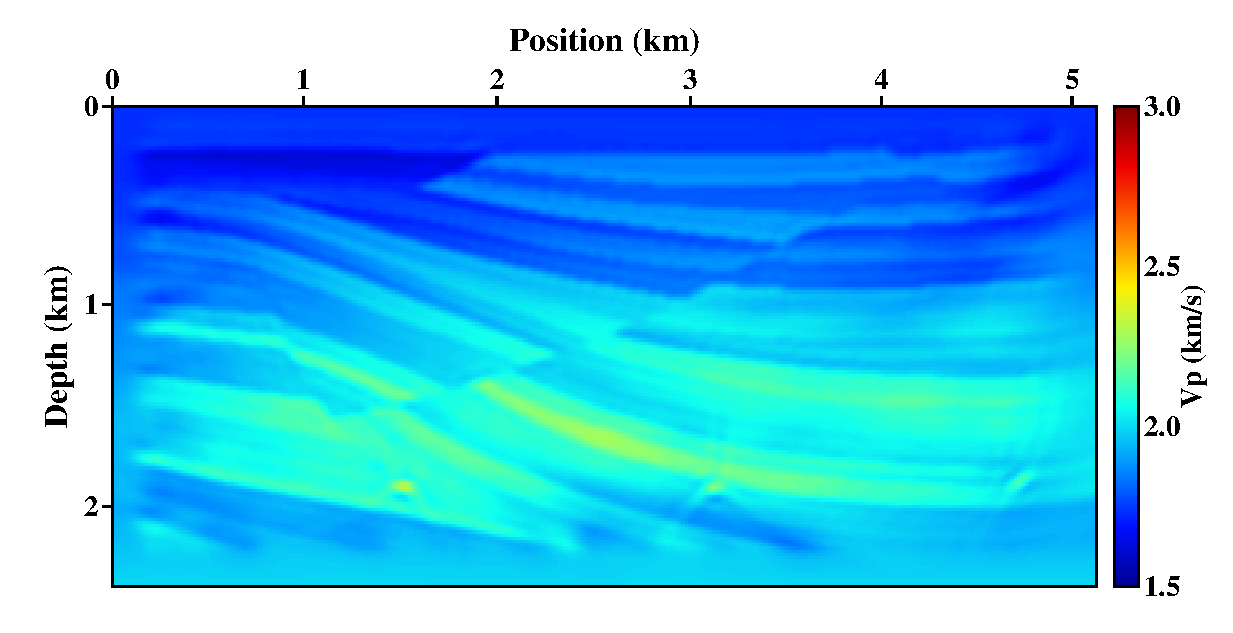
\includegraphics[width=0.45\textwidth]{sigbee2_new/Fig/EFWI_RTIvp.eps}}
   \subfigure[]{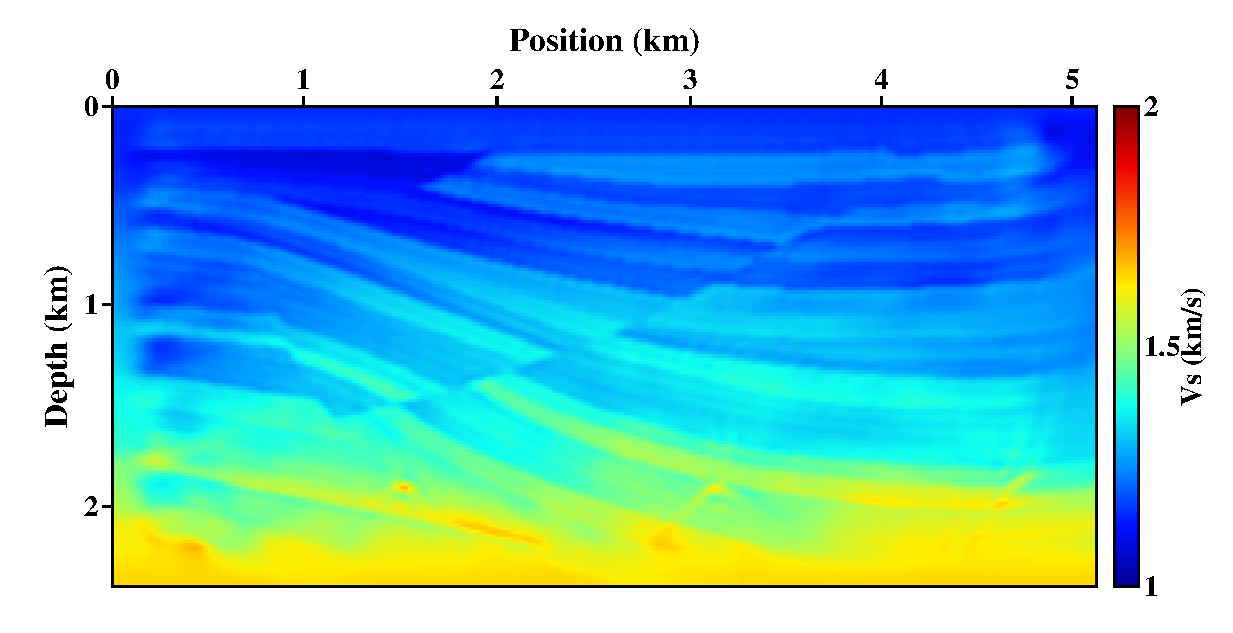
\includegraphics[width=0.45\textwidth]{sigbee2_new/Fig/EFWI_RTIvs.eps}}
   \caption{
	   EFWI results using the ERTI model as starting model. (a) $V_p$, (b) $V_s$.
%	   Inverted results of WERTI and EFWI. (a) and (b) are inverted $V_p$ and
%       $V_s$ model through two-stage elastic WERTI with the linearly increased models
%       as initial models. (c) and (d) are inverted $V_p$ and $V_s$ through EFWI using
%   (a) and (b) as starting models.
   }
   \label{fig:EWERTI+EFWI}
\end{figure}
\begin{figure}
   \centering
   \subfigure[]{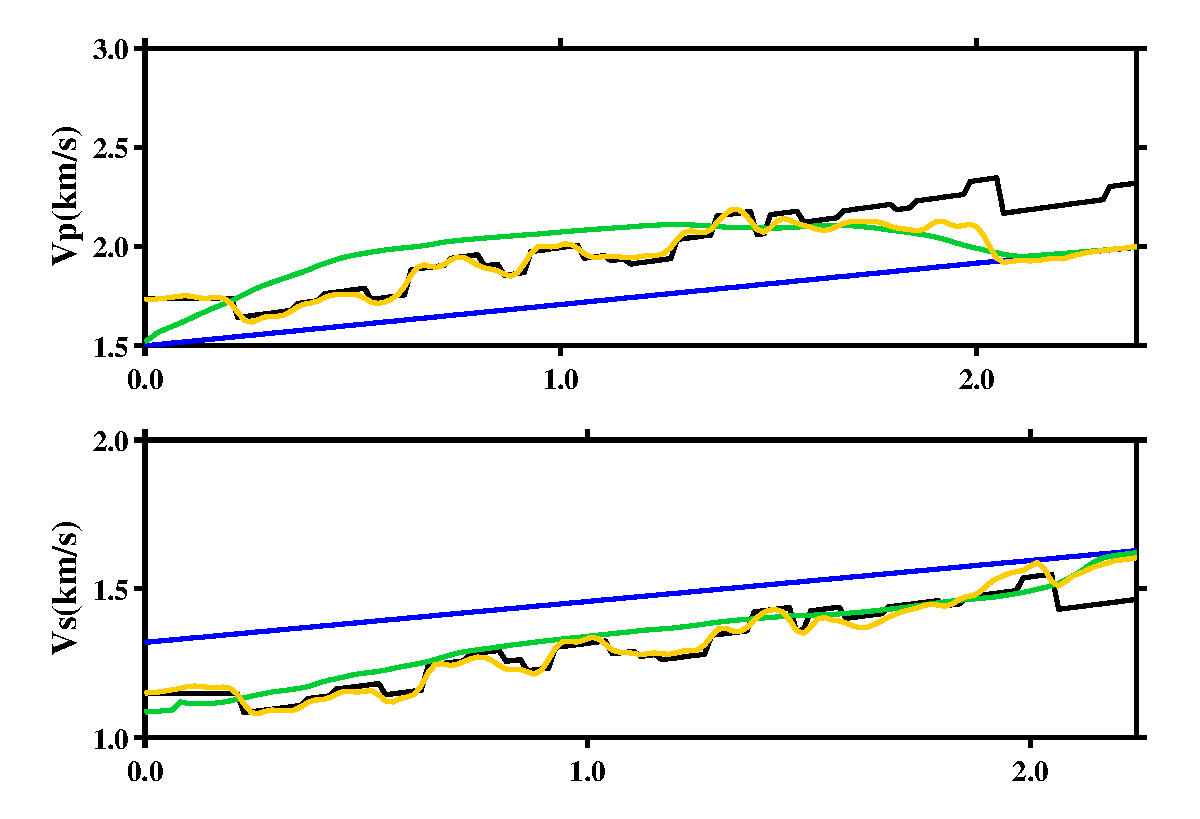
\includegraphics[width=0.45\textwidth]{sigbee2_new/Fig/1_5km.eps}}
   \subfigure[]{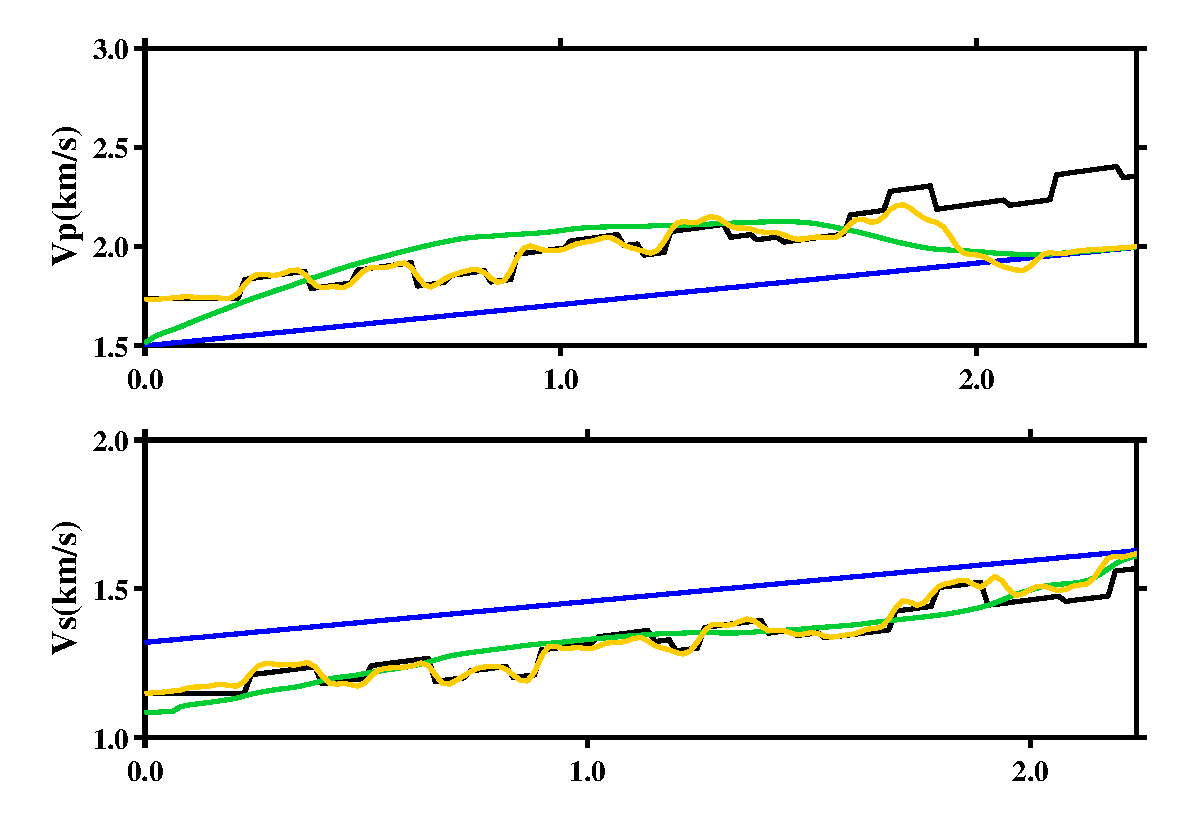
\includegraphics[width=0.45\textwidth]{sigbee2_new/Fig/3km.eps}}
   \caption{
	   Vertical profile of ERTI and EFWI model at 1.4km (a) and 3km (b).
	   The black and blue lines denote the true and initial model. The green and yellow denote
	   the ERTI and EFWI model.
%	   Vertical profiles of elastic WERTI and EFWI results at 1.4km (a) and
%       3km (b). The black and blue lines indicate the true and linearly increased
%       initial model. The green and yellow lines indicate the WERTI and EFWI results,
%       respectively.
   }
   \label{fig:Profiles}
\end{figure}
\begin{figure}
   \centering
   \subfigure[]{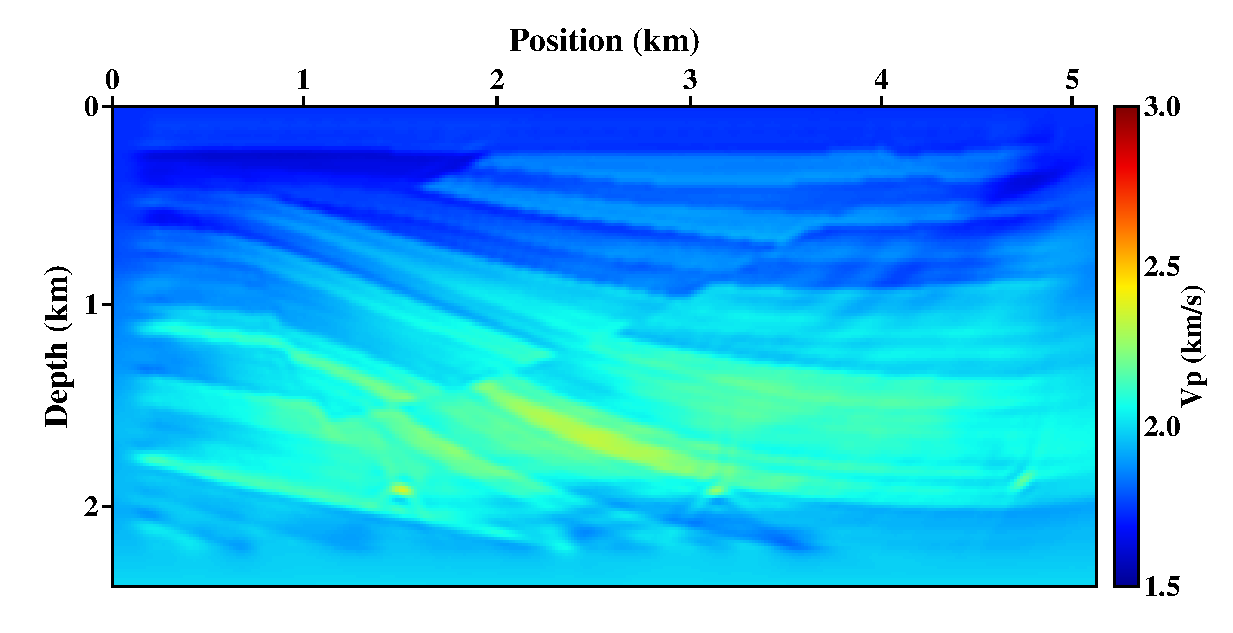
\includegraphics[width=0.45\textwidth]{sigbee2_new/Fig/Cut3Hzvp.eps}}
   \subfigure[]{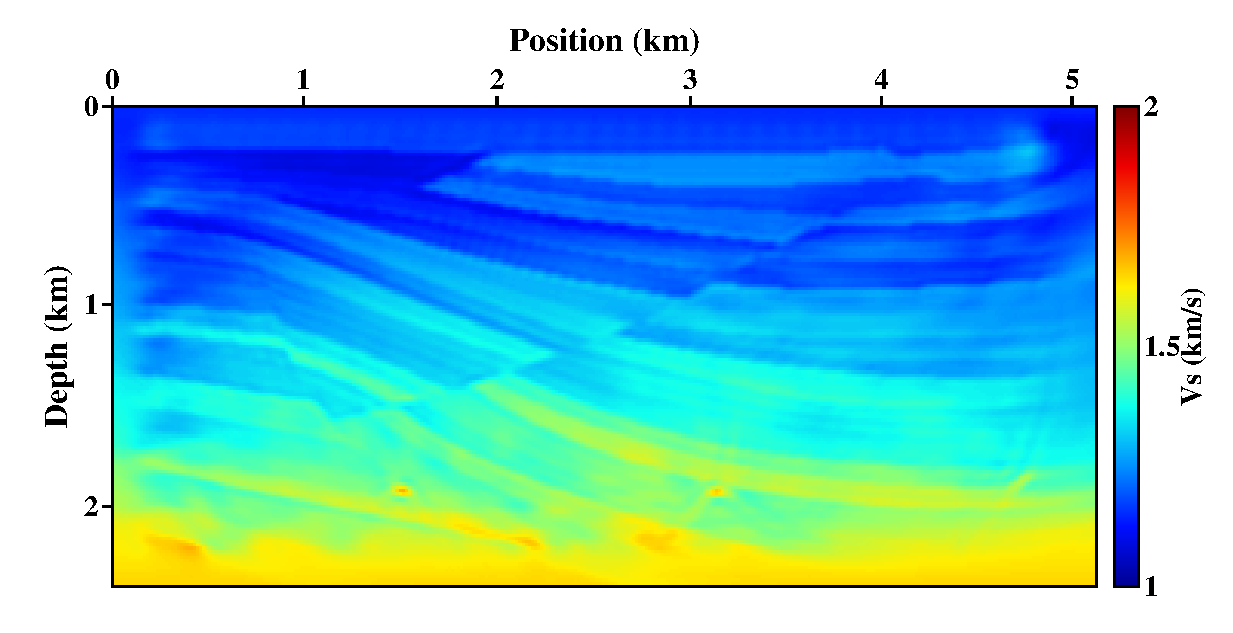
\includegraphics[width=0.45\textwidth]{sigbee2_new/Fig/Cut3Hzvs.eps}}\\
   \subfigure[]{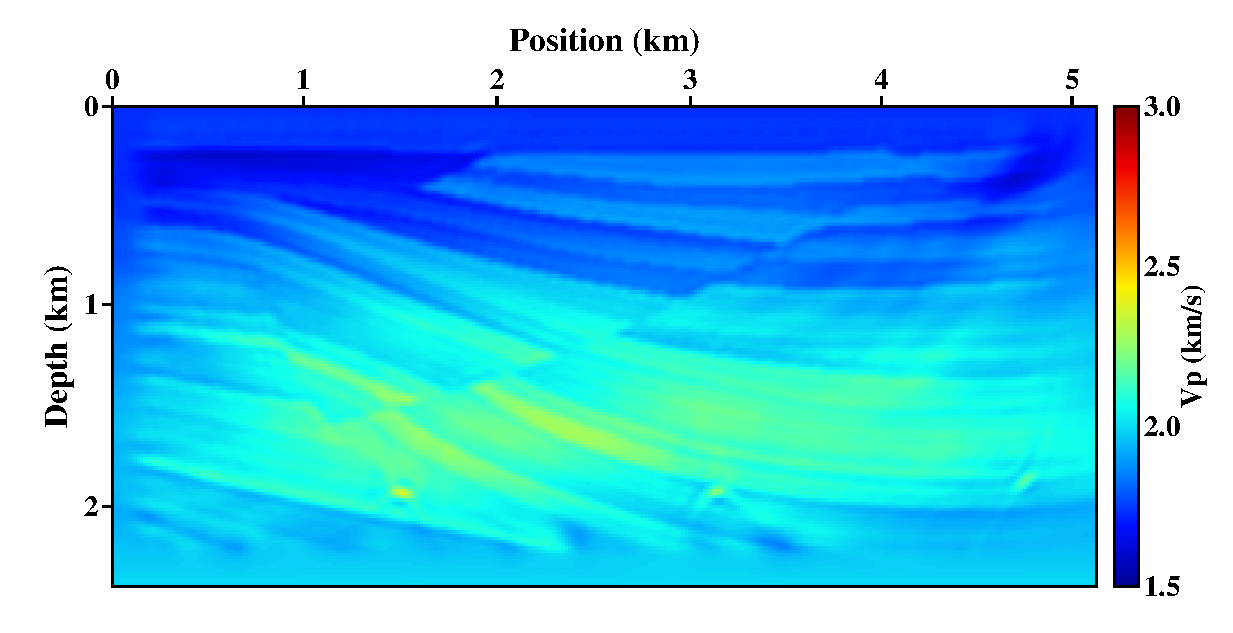
\includegraphics[width=0.45\textwidth]{sigbee2_new/Fig/Cut5Hzvp.eps}}
   \subfigure[]{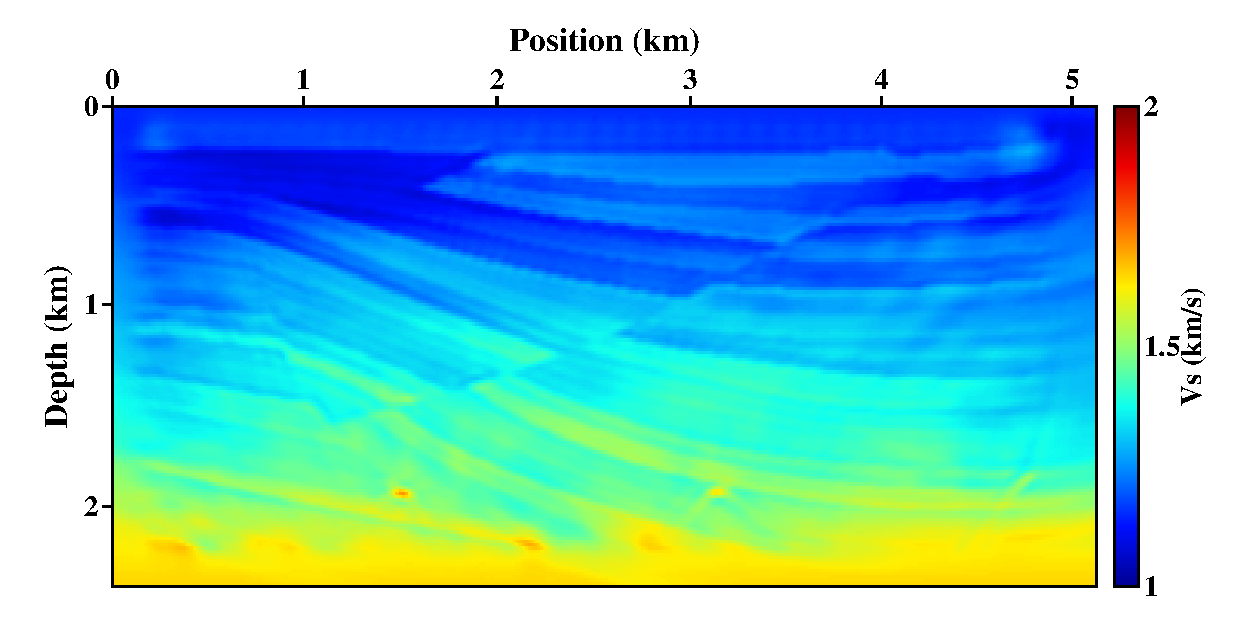
\includegraphics[width=0.45\textwidth]{sigbee2_new/Fig/Cut5Hzvs.eps}}\\
   \subfigure[]{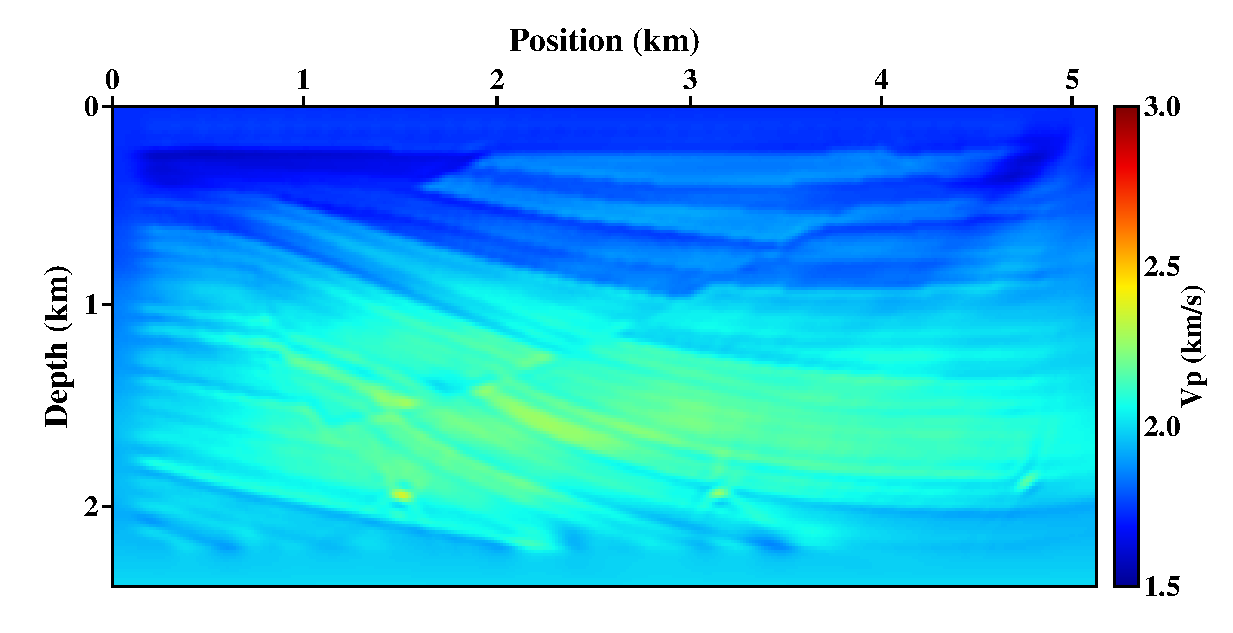
\includegraphics[width=0.45\textwidth]{sigbee2_new/Fig/Cut7Hzvp.eps}}
   \subfigure[]{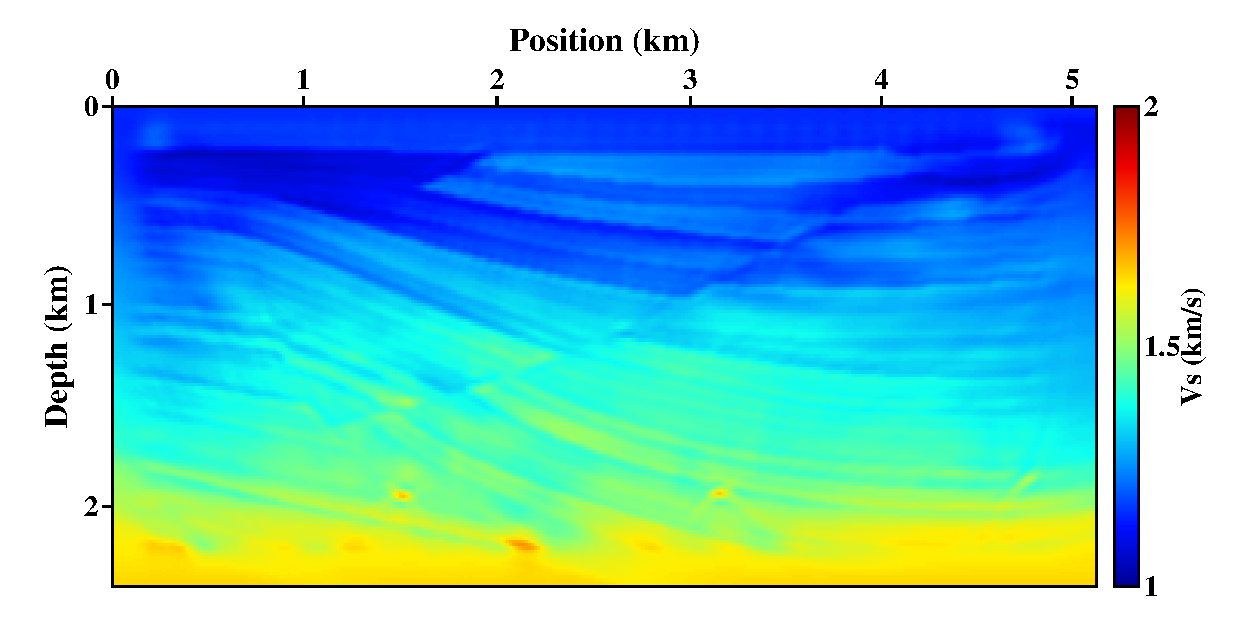
\includegraphics[width=0.45\textwidth]{sigbee2_new/Fig/Cut7Hzvs.eps}}\\
   \caption{EFWI results with different starting frequency. (a), (c), (e) are $V_p$,
   (b), (d), (f) are $V_s$.
   The starting frequency are 3Hz, 5Hz and 7Hz from top to bottom row, respectively.
   }
   \label{fig:LowFreqCut_EFWI}
\end{figure}
\clearpage
\bibliographystyle{gji}
\bibliography{reference}
\appendix
\section{Gradient derivation for ERTI with Lagrange multplier}
In this appendix, we will derive the gradients of ERTI using adjoint-state method 
\cite[]{plessix2006,Liu2006}. Accoring to \cite{Hale2013}, DIW aims to minimize the
distance between observed and calculated data:
\begin{equation}
	D(\tau)=\frac{1}{2}\int^T_0\sum_r\left[
	\mathbf{d}^c(\mathbf{x}_r,t)-
	\mathbf{d}^o(\mathbf{x}_r,t+\tau(\mathbf{x}_r,t))\right]^2dt.
        \label{eq:Dl}
\end{equation}
The optimazition of eq.\eqref{eq:Dl} satisfies:
\begin{equation}
	\frac{\partial D}{\partial \tau}=\int^T_0\sum_r
	\bsy{\alpha}(\mathbf{x}_r,t)dt=0.
        \label{eq:PartialD}
\end{equation}
where $\bsy{\alpha}(\mathbf{x}_r,t)=\dot{\mathbf{d}}^o(\mathbf{x}_r,t+\tau)(\mathbf{d}^o(\mathbf{x}_r,t+\tau)-
\mathbf{d}^c(\mathbf{x}_r,t)$.
For simpicity in derivation, we rewrite eqs \eqref{eq:WE} and \eqref{eq:DeltaWE} as:
\begin{equation}
	\begin{split}
	&\rho\partial^2_t \mathbf{u} -\bsy{\nabla\cdot}
	(\bsy{\mathbf{c}}^0\bsy{:\nabla\mathbf{u}}) = \mathbf{f}\\
	&\rho\partial^2_t
	\mathbf{\hat{u}}-\bsy{\nabla\cdot}(\bsy{\mathbf{c}}^0\bsy{:\nabla\mathbf{\hat{u}}})=
	\bsy{\nabla\cdot}(\mathbf{c}^1\bsy{:\nabla\mathbf{u}}),
	\end{split}
        \label{eq:VectorWE}
\end{equation}
where $\partial_t$ is the time derivative.
Therefore, 
using eqs \eqref{eq:VectorWE} and \eqref{eq:PartialD}
we can define the Lagrangian $\mathcal{L}$: 
\begin{equation}
	\begin{split}
		\mathcal{L}
%		(\bsy{\tau},\mathbf{u},\mathbf{\hat{u}},\bsy{\mu},
%		\bsy{\psi},\bsy{\hat{\psi}})
		&=\frac{1}{2}\sum_{r}\int^T_0\bsy{\tau}^2(\mathbf{x}_r,t)dt -\sum_{r}\int^T_0
		\bsy{\mu}(\mathbf{x}_r,t)\bsy{\alpha}(\mathbf{x}_r,t)dt\\
	&-\int^T_0\int_{\Omega} \bsy{\hat \psi}\left[\rho\partial^2_t \mathbf{u} -\bsy{\nabla
	\cdot}
	(\bsy{\mathbf{c}}^0\bsy{:}\bsy{\nabla\mathbf{u}}) - \mathbf{f}\right]d^3\mathbf{x}dt\\
	&-\int^T_0\int_{\Omega} \bsy{\psi}\left[\rho\partial^2_t
	\mathbf{\hat{u}}-\bsy{\nabla\cdot}(\bsy{\mathbf{c}}^0\bsy{:\nabla\mathbf{\hat{u}}})-
	\bsy{\nabla\cdot}(\mathbf{c}^1\bsy{:\nabla\mathbf{u}})\right]d^3\mathbf{x}dt,
	\end{split}
        \label{eq:Lagrangian}
\end{equation}
in which $\bsy{\tau}$, $\mathbf{u}$ and $\mathbf{\hat{u}}$ are state variables, 
$\Omega$ is the integration domain, 
and 
$\bsy{\mu}$, $\bsy{\psi}$ and $\bsy{\hat \psi}$ are Lagrange multipliers that need to be determined.
Note, the predicted reflection data are the wavefields observed at the receivers, i.e.,
$\mathbf{d}^c(\mathbf{x}_r,t)=\delta(\mathbf{x}-\mathbf{x}_r)\delta\mathbf{\hat{u}}$.
Here, we only consider the variation of $\mathbf{c}^0$, then the perturbation of eq.
\eqref{eq:Lagrangian} is: 
\begin{equation}
	\begin{split}
		\delta\mathcal{L}
		&=\int^T_0\sum_{r}\left[\bsy{\tau}(\mathbf{x}_r,t)-\bsy{\mu}(\mathbf{x}_r,t)\mathbf{h}(\mathbf{x}_r,t)\right]\bsy{\cdot}\delta
		\bsy{\tau}dt \\
		&+\int^T_0\int_{\Omega}
		\bsy{\mu}(\mathbf{x}_r,t)\mathbf{\dot{d}}^o(\mathbf{x}_r,t+\bsy{\tau})\delta(\mathbf{x}-\mathbf{x}_r)\bsy{\cdot}\delta
		\mathbf{\hat{u}}d^3\mathbf{x}dt\\
		&+\int^T_0\int_{\Omega}\left[
		\bsy{\hat \psi}\bsy{\nabla\cdot}(\delta \mathbf{c}^0
		\bsy{:\nabla\mathbf{u}})
		+
		\bsy{\psi}\bsy{\nabla\cdot}(\delta \mathbf{c}^0
		\bsy{:\nabla\mathbf{\hat{u}}})\right]
		d^3\mathbf{x}dt\\
	&-\int^T_0\int_{\Omega} \bsy{\hat \psi}\left[\rho\partial^2_t \delta\mathbf{u} -\bsy{\nabla
	\cdot}
	(\bsy{\mathbf{c}}^0\bsy{:\nabla\delta\mathbf{u}})\right]d^3\mathbf{x}dt\\
	&-\int^T_0\int_{\Omega} \bsy{\psi}\left[\rho\partial^2_t
	\delta\mathbf{\hat{u}}-\bsy{\nabla\cdot}(\bsy{\mathbf{c}}^0\bsy{:\nabla\delta\mathbf{\hat{u}}})-
	\bsy{\nabla\cdot}(\mathbf{c}^1\bsy{:\nabla\delta\mathbf{u}})\right]d^3\mathbf{x}dt,
	\end{split}
        \label{eq:DeltaLagrangian1}
\end{equation}
where 
$\mathbf{h}(\mathbf{x_r},t)=\dot{d}^o_i(\mathbf{x_r},t+\bsy{\tau})^2-\ddot{d}^o_i(\mathbf{x_r},t+\bsy{\tau})
(d^c_i(\mathbf{x_r},t)-d^o_i(\mathbf{x_r},t+\bsy{\tau}))$.
Upon integrating the terms involving spatial and temporal derivatives of $\mathbf{u}$,
$\delta\mathbf{u}$, $\mathbf{\hat{u}}$ and $\delta\mathbf{\hat{u}}$
%$\bsy{\psi}$ and $\bsy{\hat \psi}$ 
by parts, we have:
\begin{equation}
	\begin{split}
		\delta\mathcal{L}
		&
		=\int^T_0\sum_{r}\left[\bsy{\tau}(\mathbf{x}_r,t)-\bsy{\mu}(\mathbf{x}_r,t)\mathbf{h}(\mathbf{x}_r,t)\right]\bsy{\cdot}\delta
		\bsy{\tau}dt \\
		& +\int^T_0\int_{\Omega}
		\bsy{\mu}(\mathbf{x}_r,t)\mathbf{\dot{d}}^o(\mathbf{x}_r,t+\bsy{\tau})\delta(\mathbf{x}-\mathbf{x}_r)\bsy{\cdot}\delta
		\mathbf{\hat{u}}d^3\mathbf{x}dt\\
		& -\int^T_0\int_{\Omega}\left[
		\bsy{\nabla\hat \psi:}\delta \bsy{\mathbf{c}}^0\bsy{:\nabla\mathbf{u}})
		+\bsy{\nabla\psi:}\delta \bsy{\mathbf{c}}^0\bsy{: \nabla\mathbf{\hat{u}}})\right]
		d^3\mathbf{x}dt\\
		& -\int^T_0\int_{\Omega} \left[\rho\partial^2_t \bsy{\hat \psi} -\bsy{\nabla
		\cdot}	(\bsy{\mathbf{c}}^0\bsy{:\nabla\bsy{\hat
		\psi}})-\bsy{\nabla\cdot}(\bsy{\mathbf{c}}^1\bsy{:\nabla\psi})
		\right]\delta\mathbf{u}d^3\mathbf{x}dt\\
	&-\int^T_0\int_{\Omega} \left[\rho\partial^2_t
	\bsy\psi-\bsy{\nabla\cdot}(\bsy{\mathbf{c}}^0\bsy{:\nabla\bsy\psi})\right]
	\delta\mathbf{\hat{u}}d^3\mathbf{x}dt\\
	&-\int_{\Omega} [\rho(\bsy{\hat \psi}
	\bsy{\cdot}\partial_t\delta\mathbf{u}-\partial_t\bsy{\hat \psi}\bsy{\cdot}\delta\mathbf{u}
	+\bsy{\psi}\bsy{\cdot}\partial_t\delta\mathbf{\hat{u}}-\partial_t
	\bsy{\psi}\bsy{\cdot}\delta\mathbf{\hat{u}})]^T_0d^3\mathbf{x}	\\
	&+\int^T_0\int_{\partial\Omega} \bsy{\hat
	\psi}\bsy{\cdot}[\mathbf{n}\bsy{\cdot}(\delta\mathbf{c}^0:\bsy{\nabla}\mathbf{u}+\mathbf{c}^0:\bsy{\nabla}\delta\mathbf{u})]
	-\mathbf{n}\bsy{\cdot}(\mathbf{c}^0:\bsy{\nabla}\bsy{\hat \psi})\bsy{\cdot}\delta\mathbf{u}d^2\mathbf{x}dt\\
	&+\int^T_0\int_{\partial\Omega} \bsy{
	\psi}\bsy{\cdot}[\mathbf{n}\bsy{\cdot}(\delta\mathbf{c}^0:\bsy{\nabla}\mathbf{\hat{u}}+\mathbf{c}^0:\bsy{\nabla}\delta\mathbf{\hat{u}})]
	-\mathbf{n}\bsy{\cdot}(\mathbf{c}^0:\bsy{\nabla}\bsy{\psi})\bsy{\cdot}\delta\mathbf{\hat{u}}d^2\mathbf{x}dt\\
	&+\int^T_0\int_{\partial\Omega} \bsy{
	\psi}\bsy{\cdot}[\mathbf{n}\bsy{\cdot}(\mathbf{c}^1:\bsy{\nabla}\delta\mathbf{u})]
	-\mathbf{n}\bsy{\cdot}(\mathbf{c}^1:\bsy{\nabla}\bsy{\psi})\bsy{\cdot}\delta\mathbf{u}d^2\mathbf{x}dt
	\end{split}
        \label{eq:DeltaLagrangian2}
\end{equation}
where $\mathbf{n}$ is the unit outward vector normal on the surface
$\partial\Omega$. The displacement wavefields (state variables) are subject to the initial and boundary condition:
\begin{equation}
	\begin{split}
	&\mathbf{u}(\mathbf{x},0)=0,\partial_t\mathbf{u}(\mathbf{x},0)=0,
	\mathbf{u}(\mathbf{x},t)\rvert_{x\rightarrow\infty}\to0\\
	&\mathbf{\hat{u}}(\mathbf{x},0)=0,\partial_t\mathbf{\hat{u}}(\mathbf{x},0)=0,
	\mathbf{\hat{u}}(\mathbf{x},t)\rvert_{x\rightarrow\infty}\to0
	\end{split}
        \label{eq:InitialBoundary}
\end{equation}
while the adjoint state variables satisfy the ``final'' (at Time $T$) and boundary condition:
\begin{equation}
	\begin{split}
	&\bsy{\psi}(\mathbf{x},T)=0,\partial_t\bsy{\psi}(\mathbf{x},T)=0,
	\bsy{\psi}(\mathbf{x},t)\rvert_{x\rightarrow\infty}\to0\\
	&\bsy{\hat\psi}(\mathbf{x},T)=0,\partial_t\bsy{\hat{\psi}}(\mathbf{x},T)=0,
	\bsy{\hat{\psi}}(\mathbf{x},t)\rvert_{x\rightarrow\infty}\to0
	\end{split}
        \label{eq:InitialBoundary_2}
\end{equation}
Thus all the surface integrals in eq.\eqref{eq:DeltaLagrangian2} will disappear, then:
\begin{equation}
	\begin{split}
		\delta\mathcal{L}
		&
		=\int^T_0\sum_{r}\left[\bsy{\tau}(\mathbf{x}_r,t)-\bsy{\mu}(\mathbf{x}_r,t)\mathbf{h}(\mathbf{x}_r,t)\right]\delta
		\bsy{\tau}dt \\
		& -\int^T_0\int_{\Omega} \left[\rho\partial^2_t \bsy{\hat \psi} -\bsy{\nabla
		\cdot}	(\bsy{\mathbf{c}}^0\bsy{:\nabla\bsy{\hat
		\psi}})-\bsy{\nabla\cdot}(\bsy{\mathbf{c}}^1\bsy{:\nabla\psi})
		\right]\delta\mathbf{u}d^3\mathbf{x}dt\\
		&
		-\int^T_0\int_{\Omega}\left[\rho\partial^2_t\bsy\psi-\bsy{\nabla\cdot}(\bsy{\mathbf{c}}^0\bsy{:\nabla\bsy\psi})-
		\bsy{\mu}(\mathbf{x}_r,t)\mathbf{\dot{d}}^o(\mathbf{x}_r,t+\bsy{\tau})\delta(\mathbf{x}-\mathbf{x}_r)\right]\delta
		\mathbf{\hat{u}}d^3\mathbf{x}dt\\
		& -\int^T_0\int_{\Omega}\left[
		\bsy{\nabla\hat \psi:}\delta \bsy{\mathbf{c}}^0\bsy{:\nabla\mathbf{u}})
		+\bsy{\nabla\psi:}\delta \bsy{\mathbf{c}}^0\bsy{: \nabla\mathbf{\hat{u}}})\right]
		d^3\mathbf{x}dt.
	\end{split}
        \label{eq:DeltaLagrangian3}
\end{equation}
To obtain the stationary point, setting the coeffients of $\delta \bsy{\tau}$ to zero yields:
\begin{equation}
	\bsy{\tau}(\mathbf{x}_r,t)-\bsy{\mu}(\mathbf{x}_r,t)\mathbf{h}(\mathbf{x}_r,t)
	=0,
        \label{eq:Adjoint1}
\end{equation}
and setting 
$\delta \mathbf{u}$
and $\delta \mathbf{\hat{u}}$ to zero yields another two adjoit state equations:  
\begin{equation}
	\begin{split}
	&\rho\partial^2_t
	\bsy\psi-\bsy{\nabla\cdot}(\bsy{\mathbf{c}}^0\bsy{:\nabla\bsy\psi})
	=\bsy{\mu}(\mathbf{x}_r,t)\mathbf{\dot{d}}^o(\mathbf{x}_r,t+\bsy{\tau})\delta(\mathbf{x}-\mathbf{x}_r),\\
	&\rho\partial^2_t \bsy{\hat \psi} -\bsy{\nabla\cdot}
	(\bsy{\mathbf{c}}^0\bsy{:\nabla\bsy{\hat
	\psi}})=\bsy{\nabla\cdot}(\bsy{\mathbf{c}}^1\bsy{:\nabla\psi}).
	\end{split}
        \label{eq:AdjointAll}
\end{equation}
The adjoint sources are different in the above equations.
The first line represents that the adjoint background wavefields $\bsy{\psi}$ is determined
by a new adjoint source at the receiver locations. While the second line represents that the perturbed adjoint wavefields
$\bsy{\hat \psi}$ is determined by the virtual source generated by the high-wavenumber image perturbations.
The adjoint wavefields $\bsy{\psi}$ and $\bsy{\hat \psi}$ can be obtained by solving eq.\eqref{eq:AdjointAll} in a time-reversed
manner. Then, the gradient
is: 
\begin{equation}
	\frac{\partial \mathcal{L}}{\partial \mathbf{c}^0}=-\int^T_0\int_{\Omega}\left[\bsy{\nabla\hat \psi} \bsy{\nabla\mathbf{u}}+
	\bsy{\nabla\psi}\bsy{\nabla\mathbf{\hat{u}}}\right]d^3\mathbf{x}dt,
\end{equation}
or in a more detailed manner:
\begin{equation}
	\frac{\partial E}{\partial c^0_{ijkl}}=-\int (\frac{\partial u_{i}}{\partial
	x_j}\frac{\partial \hat \psi_{k}}{\partial x_l}+\frac{\partial \hat{u}_{i}}{\partial
	x_j}\frac{\partial \psi_{k}}{\partial x_l}),
    \label{eq:GradientCijkl_app}
\end{equation}

\section{Further decomposition of $V_s$ reflection kernels}
In the previously section, we give the further decomposition of Fig. \ref{fig:kernel_vs_decomp}h. Here, we will
investigate the decomposition of the rest three parts, i.e. Figs
\ref{fig:kernel_vs_decomp}e-g.
Fig. \ref{fig:kernel_vs_src} show the decomposition of two source terms. 
When only injecting PP data, the wavefield $\bsy{\psi}^{PP-S}$ 
will occur due to the non-physical mode conversions.
In $\bsy{\psi}^{PP-S}$, PP indicates the injection data while S indicates the conversion type at receiver.
The same definition is used in the following context.
For simplicity, we only label the figure with $\bsy{\psi}$ to represent the background wavefields 
back-propagated in the media.
Mode conversions will produce different type
of migration impulse at the source side. 
It is easy to recognize the PP wavepath shown in Fig. \ref{fig:kernel_vs_src}e. 
While the cross-mode correlation produces high-wavenumber energy near the interface. 
When only injecting PS data, the $\psi^{PS-P}$ will occur as well.
Fig. \ref{fig:kernel_vs_src}g shows a similar case as the Fig. \ref{fig:kernel_vp_decomp}f.
Note, in \ref{fig:kernel_vs_src}h there are 
two migration impulse because two type of S-wave conversions exist in $\boldsymbol{\hat\psi}$. Fisrt,
the normal $\boldsymbol{\psi}^{PS}$ wavefield produce a S-wave reflection $\boldsymbol{\psi}^{PS-S}$
when incidenting at the interface. Second, the injection-induced non-physical conversion at receiver
$\boldsymbol{\psi}^{PS-P}$ also generates a S-wave conversion $\boldsymbol{\psi}^{PS-P-S}$. 
Separating the above two migration impulses is possible but requires more efforts and calculations in which one
should separate the wavefields $\boldsymbol{\psi}$ into $\boldsymbol{\psi}^{PS}$ and $\boldsymbol{\psi}^{PS-P}$ in
demigration (solving eq.\eqref{eq:AdjointDeltaWE}). 

Finally, we decompose the kernel in Fig. \ref{fig:kernel_vs_decomp}g.
Only PP data is injected. The non-physical conversions at receiver are highlighted as red. 
Fig. \ref{fig:kernel_vs_recPP}c shows the component of PP reflection wavepath.
We can see the cross-mode correlations produce high-wave number energy near the interface or around the
receiver location ( Figs \ref{fig:kernel_vs_recPP}d and e).
In Fig. \ref{fig:kernel_vs_recPP}f,
there is no energy in the SS-mode component. One plausible reason is that the two S-wavefields do
not meet with each other to give a migration impulse due to the inconsistency of traveltime. 
\begin{figure}
   \centering
   {\includegraphics[width=1.0\textwidth]{Kernel/Combinations/K_vs_src_new.eps}}
   \caption{
   Further decomposed components of Fig \ref{fig:kernel_vs_decomp}e and
   \ref{fig:kernel_vs_decomp}f. (a) The PP data for adjoint source
   , (b) Source side of $K_{V_s}$ using (a) as adjoint source, 
   (c) The PS data for adjoint source,
   (d) Source side of $K_{V_s}$ using (c) as adjoint source, 
   (e)-(h): 
   The first line denotes the manner and wavefield type for cross-correlation.
   The second line denotes the corresponding kernels.
   }
   \label{fig:kernel_vs_src}
\end{figure}
\begin{figure}
   \centering
   {\includegraphics[width=1.0\textwidth]{Kernel/Combinations/K_vs_recPP_new.eps}}
   \caption{Further decomposed components of Fig \ref{fig:kernel_vs_decomp}g. (a) The adjoint source
   for injection, (b) Receiver term of $K_{V_s}$ using (a) as adjoint source, (c)-(f) 
   The first line denotes the manner and wavefield type for cross-correlation.
   The second line denotes the corresponding kernels.
   }
   \label{fig:kernel_vs_recPP}
\end{figure}
\section{problems in PS demigration}
Under the high-frequency approximation, we will illustrate the difference between method
\Rome{1} and \Rome{2} when
predicting the PS reflection.
A single reflector example is adopted to show the inappropriate behavior of method
\Rome{1} for inversion through 
map migration and demigration.

%A slight deviation of $V_p$ around the true value will lead
%to a wrongly traveltime residual of PS reflection. However, method
%{\bf\uppercase\expandafter{\romannumeral2}} can provide correct traveltime residuals. 

%Since the PS reflection is asymmetric, the ray path of PS is shown in 
Fig. \ref{fig:PS_refl} shows the asymmetric ray path of PS reflection.
According to the Snell's law and geometrical relationship, we have:
\begin{equation}
\begin{split}
    &\frac{sin\theta_1}{V_p}=\frac{sin\theta_2}{V_s},\\
	&z(tan\theta_1+tan\theta_2)=X,
\end{split}
    \label{eq:Snell_PS} 
\end{equation}
with $V_p$ and $V_s$ are the correct velocity, $X$ is the offset, $z$ is the depth, 
and $\theta_1$ and $\theta_2$ are the incident and reflected angles, respectively.
Therefore, the moveout of PS reflection is:
\begin{equation}
	t=\frac{z}{cos\theta_1V_p}+\frac{z}{cos\theta_2V_s}.
    \label{eq:TravelTime_PS} 
\end{equation}
The difference between method \Rome{1} and \Rome{2} 
is the migrated depth when velocity model is inaccurate. 
However, the zero offset map migration for PS data is impossible because PS conversion
at near offset is very weak. The energy of near offsets PS data imaging mainly consists of
the reflection from certain angles. Therefore, we should use the finite offset map
migration to determine the migrated depth. 

In method \Rome{1}, the finite offset map migration is illustrated by Fig.
\ref{fig:PS_refl}, the migrated depth ($z_{1}$) satisfies:
\begin{equation}
	\begin{split}
	&\frac{z_{1}}{cos\alpha_2V^{'}_p}+\frac{z_{1}}{cos\alpha_2V^{'}_s}=\frac{z}{cos\theta_1V_p}+\frac{z}{cos\theta_2V_s},\\
	&z_{1}(tan\alpha_1+tan\alpha_2)=z(tan\theta_1+tan\theta_2).\\
	&\frac{sin\alpha_1}{V^{'}_p}=\frac{sin\alpha_2}{V^{'}_s},\\
	\end{split}
	\label{eq:Mapmigration_PS} 
\end{equation}
where $V^{'}_p$ and $V^{'}_s$ are the wrong velocity, $\alpha_1$ and $\alpha_2$ are
the incident and reflected angles, respectively, when velocity is wrong. Given a
certain incident angle $\theta_1$, we can calculate the migration depth combining eqs
\eqref{eq:Snell_PS} and \eqref{eq:Mapmigration_PS}.
%Generally, $V_p>V_s$ and $V^{'}_p>V^{'}_s$. Therefore, a small perturbation of
%$V^{'}_p$ will lead to a relatively big change of $\frac{V_p+V_s}{V^{'}_p+V^{'}_s}$, which
%means that the migration depth $z_{1}$ is very sensitive to both $V^{'}_p$ and $V^{'}_s$. 
While in method \Rome{2}, we can use the zero offset map migration. Easily, the depth after migration is: 
\begin{equation}
	{z_{2}}=\frac{V^{'}_p}{V_p}z.
    \label{eq:ZerooffMig_PP} 
\end{equation}
Then, we use this depth and the
wrong velocity through equation \eqref{eq:TravelTime_PS} to predict the traveltime of PS reflection.
%Then, the demigration process can be implemented with:
%\begin{equation}
%	t^{'}=\frac{z^{'}}{cos\theta_1V^{'}_p}+\frac{z^{'}}{cos\theta_2V^{'}_s}.
%    \label{eq:Demigration_PS} 
%\end{equation}
%where $z^{'}\in\{z_1,z_2\}$ is the migrated depth and $t^{'}$ is the corresponding
%demigrated two-way traveltime.

To show the differences, we compare the predicted traveltime
curves of the two methods with the observed ones.
Here, $V_p=2500m/s$, $V_s=1500m/s$, $V^{'}_s=1300m/s$ are fixed and the value of $V^{'}_p$
are assumed to be correct ($2500m/s$). We assume the depth of reflector is 1000m, the
incident angle is $\theta_1=10^{\circ}$ (offset 281m)
As shown in Figure \ref{fig:Sens_vp}a, 
the predicted PS traveltime with method
\Rome{1} (black) is below the true value (red) at large offset, which is consistent
with the velocity error. However, at the near offset (Fig.\ref{fig:Sens_vp}b), the predicted traveltime is
above the true one. 
This will lead to an negative update of the S-wave velocity even the $V^{'}_s$ is
lower than the true one.
In this case, the PS demigration with method \Rome{1} 
would give a wrong estimation of traveltime residual at near offset.
If the incident angle (offset) is smaller, the vertex of the black line will descend
until to a ``kissing point'' when incident angle is zero (green line).
Here, we use the ray theory to assume a zero-offset map migration of PS data, but the
zero offset data of PS reflection is inavailable in real case.
%indicating a wrong sign of the traveltime residual because $V^{'}_s$ is lower than the true one. 
%Theoretically, the predicted
%curve should behave like the second black line ($V^{'}_p=V_p$), where the zero-offset traveltime is correct while
%the long offset traveltime is larger than the true one. Note, when $V^{'}_p=2450m/s$, the
%predicted curve is inconsistent with the S-wave velocity error
%($V^{'}_s<V_s$). While when $V^{'}_p=2550m/s$ the predicted curve is below the true value. 
%This means that the sign of the traveltime residual will be very sensitive to the error of $V_p$ model,  
%even if the error of $V_p$ is as small as $\pm50m/s$. 
%If the depth of reflector decreases, the sensitivity of method \Rome{1} reduces (figure \ref{fig:Sens_vp}b). But the
%inconsistency between residual and velocity error still exists, especailly in the small offset.
%This kind of sign change leads to 
%the abnormal change of the gradient's direction during the inversion. 
Therefore, the nonlinearity of inversion increases obviously due to this wrong
estimation. 
Fortunately, if we use method \Rome{2},
the predicted curves (blue) are all below the true value, whose traveltime residual are consistent
with the S-wave velocity error.
%However,
%method \Rome{2} also provides correct time residuals as the previous one.
According to the above analysis, we recommend method \Rome{2} to implement the PS stage inversion.
\clearpage
\begin{figure}
   \centering
%   \subfigure[]{\includegraphics[width=0.40\textwidth]{PS_problem/PS_refl.eps}}
   \subfigure{\includegraphics[width=0.40\textwidth]{PS_problem/PS_refl_mapmigration.eps}}
   \caption{Schematic illustration of PS reflection ray path and its finite offset map
   migration. The solid line indicates the ray path of PS
   reflection with a single reflector. The dashed line indicates the finite offset map migration when velocity is wrong.}
   \label{fig:PS_refl}
\end{figure}
\begin{figure}
   \centering
   \subfigure[]{\includegraphics[width=0.45\textwidth]{PS_problem/PS_refl_new.eps}}
   \subfigure[]{\includegraphics[width=0.45\textwidth]{PS_problem/PS_refl_new_zoomin.eps}}
   \caption{The comparison among demigrated PS traveltime moveout of method \Rome{1}
   (black, green), method 
   \Rome{2} (blue) and the real (red) one.
   The black and green lines represents the results of $\theta_1=10^{\circ}$ and
   $\theta_1=0^{\circ}$, respectively.
   (a) the original curves, (b) the curves in the dash box in (a).}
   \label{fig:Sens_vp}
\end{figure}

\end{document}
